\chapter{详细设计与实现}

本章将详细拆解系统的具体实现过程，核心逻辑是将工程落地与前期的研究方向深度绑定。针对AI任务配性差的痛点，本工作在API接入层与执行层建立了参数画像与自动纠偏机制，把繁琐的人工纠错转化成了系统的自动化本能；为了解决调度决策太依赖人工的问题，调度层引入了环境感知的自动决策引擎；而针对GPU等贵重资源出现占用冲突所引发的效率瓶颈，本系统通过互斥分析算法实现了从低效串行到高效并发的质变。这些技术实现不仅让系统能看懂AI任务，更从底层保障了多任务场景下的算力利用率与运行稳健性。

\section{API接入层详细设计}

API接入层作为系统的首要入口，承担着用户指令进入调度中枢的唯一通道角色。该层通过整合Docker容器化环境、服务治理组件及FastAPI异步框架，构建了稳固的运行基础设施，其设计核心聚焦于安全性与鲁棒性，分别由权限鉴定与数据校验两大模块负责，确保所有AI调度指令具备合法性与可靠性。

在研究方向的关联上，该层是解决AI适配性欠佳的关键环节。针对AI大模型任务参数复杂、人工录入易出错的痛点，本文利用数据校验模块建立了严密的参数画像与自动化纠偏逻辑，将以往因类型不符或格式错误所引发的系统崩溃问题，在接入端通过技术手段予以消除，显著提升了系统对异构AI数据的处理能力。同时，严密的权限鉴定机制确保了仅授权任务可调用昂贵的GPU算力，为后续调度层在纯净、安全的数据环境下解决“自动化决策”与“资源互斥分析”问题奠定了坚实基础。

\subsection{权限鉴定模块}

安全性在本系统中不仅是基础的准入要求，更是支撑AI多任务调度的前置屏障。在AI大模型研发场景下，GPU等算力资源不仅稀缺，且租赁成本极高，任何未经授权的调用或非法的任务下发，都将直接导致昂贵计算资源的无效空耗。尽管系统部署于公司内网，但在数万员工协同工作的大型环境下，内网身份并不等同于操作可信。因此，引入严格的身份认证机制，是防范资源误用的首要措施。

针对本文所研究的多任务场景，本工作引入了“任务组”隔离机制：通过对用户角色与任务组进行M:N的关系映射，确保操作员只能在被授权的业务范围内创建、修改或撤销任务。该设计深度契合研究背景中对“资源浪费”的治理需求，通过权限锁定，从源头上杜绝因跨团队误操作而引发的任务冲突或算力抢占。这不仅保障了数据的私密性，也为后续调度层执行“资源互斥分析”提供了纯净且可控的初始状态，从而确保系统在复杂环境下依然能够维持高度的稳定性。其主要流程如图5.1所示。

\begin{figure}[htbp]
    \centering
    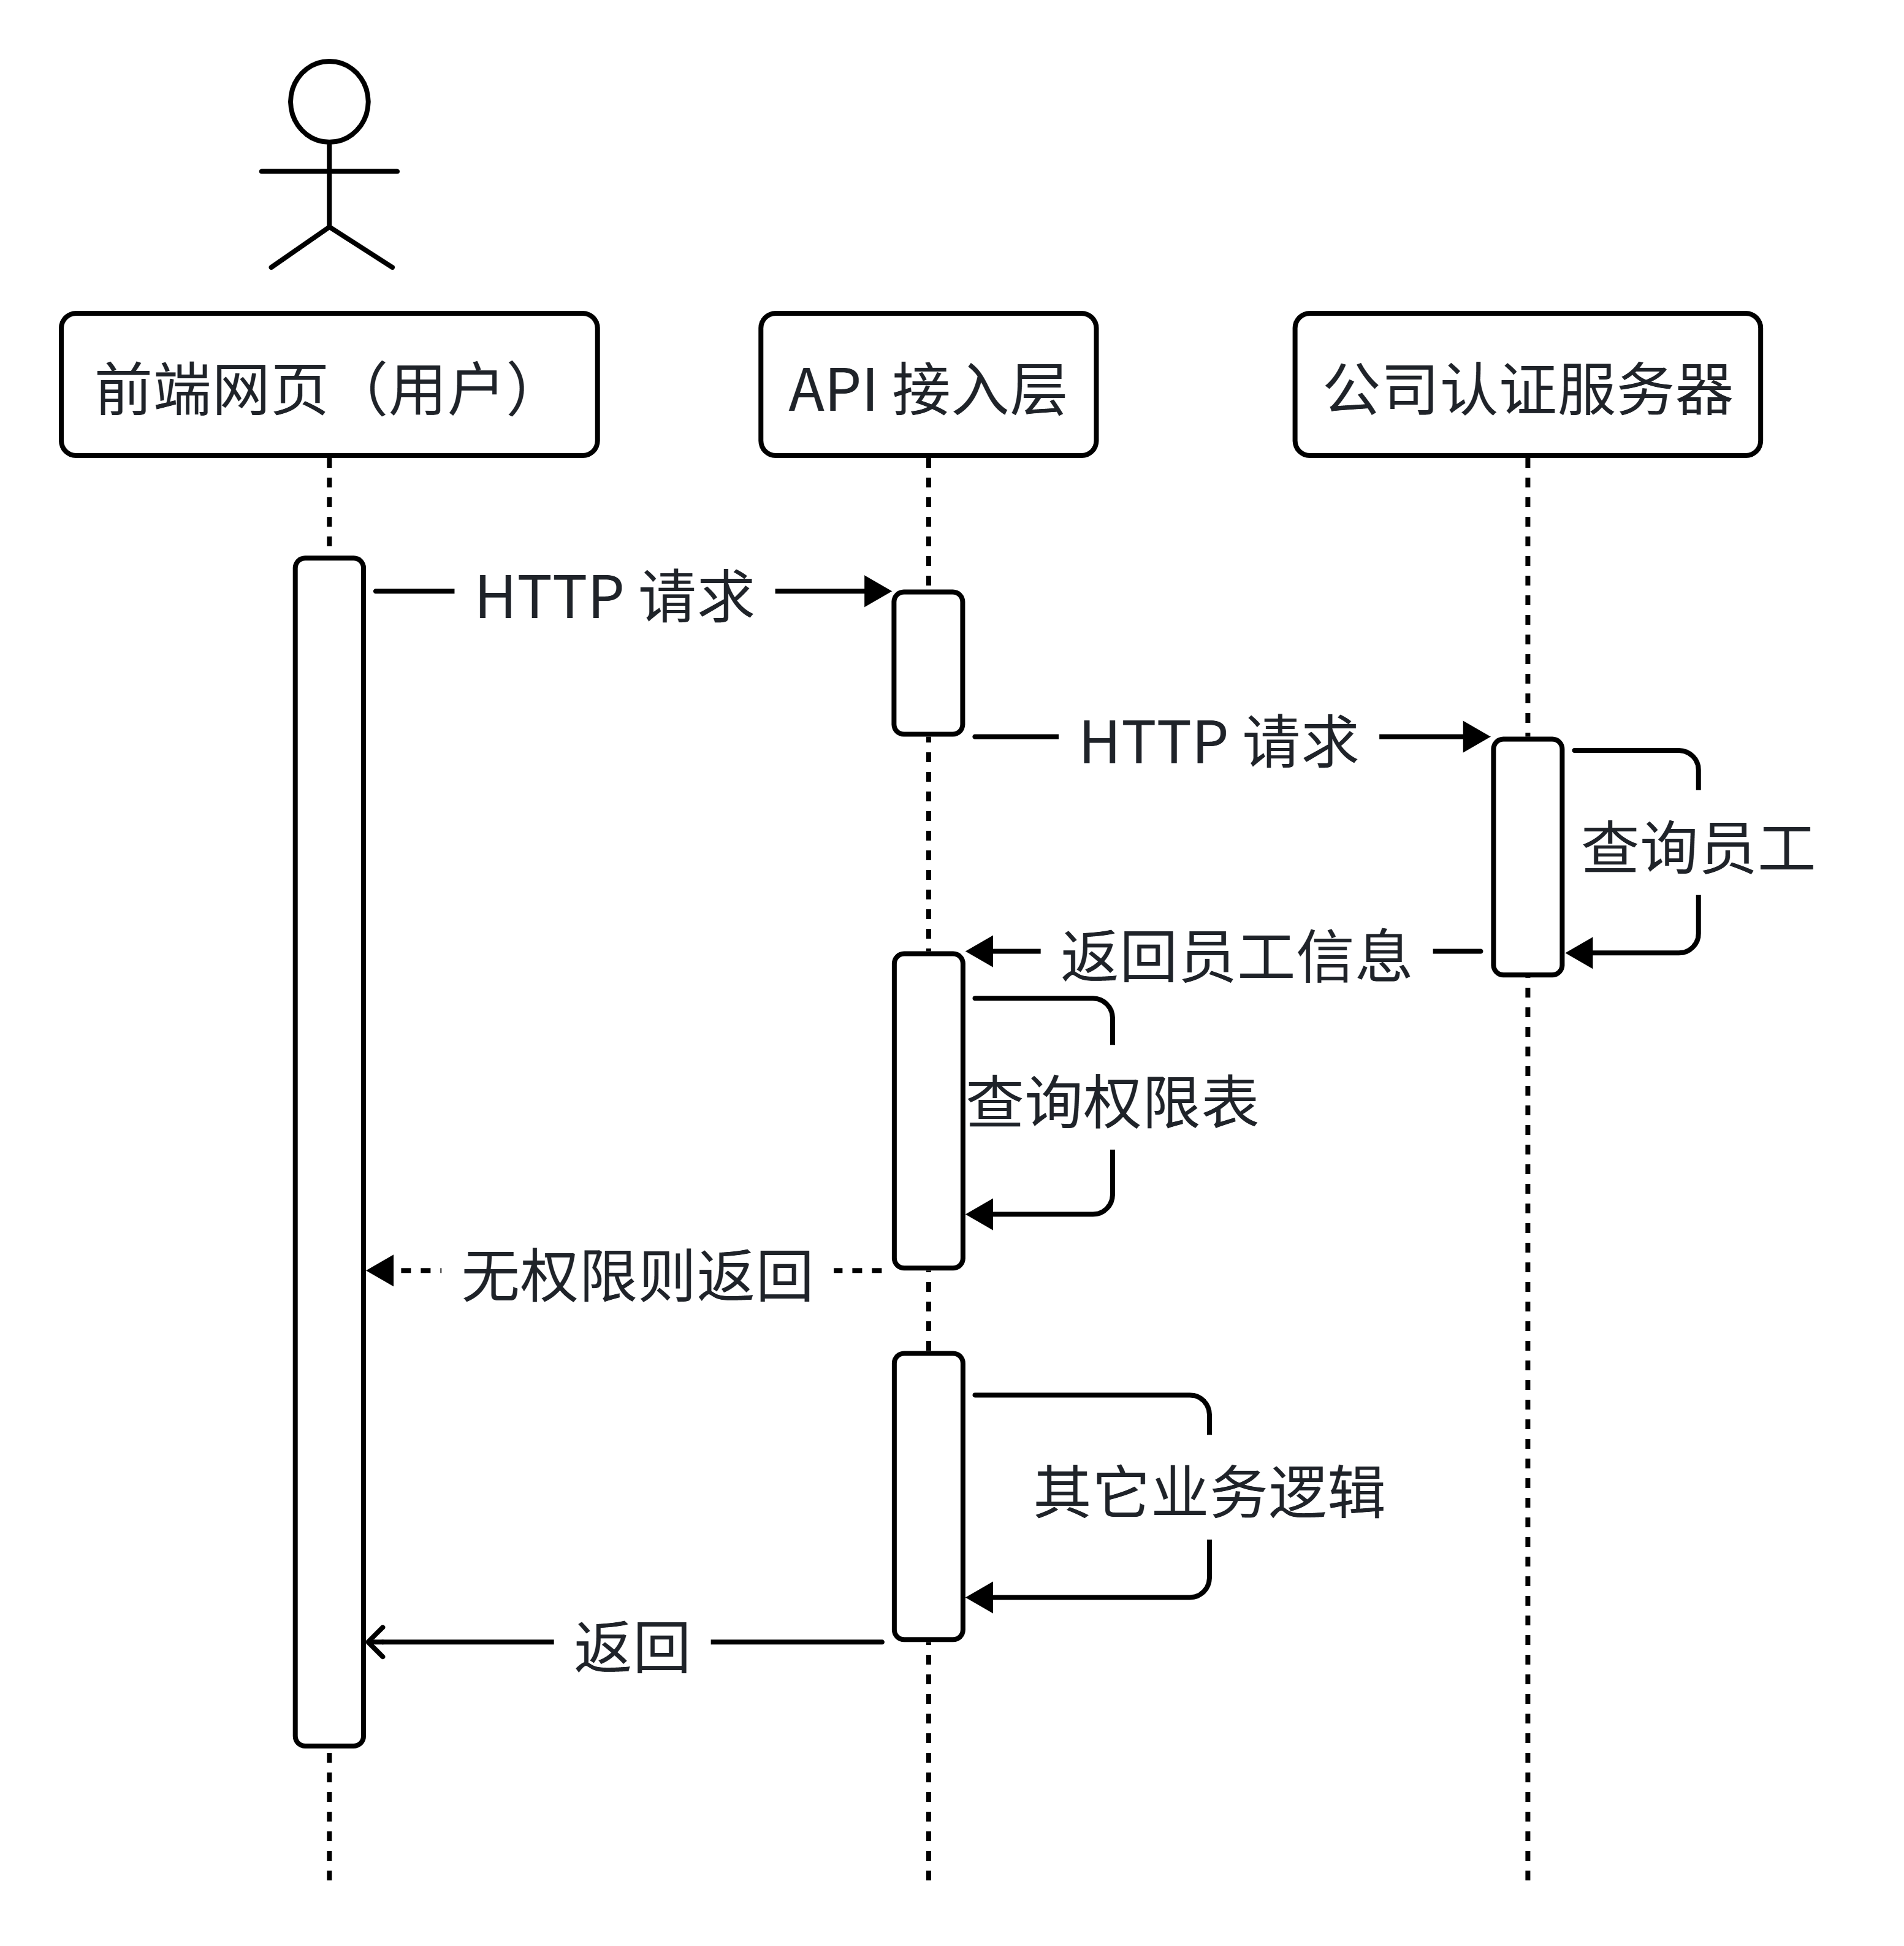
\includegraphics[width=0.8\linewidth]{figures/5/权限鉴定流程.png}
    \caption{权限鉴定时序图}
    \label{fig:enter-label}
\end{figure}

用户通过前端网页发起HTTP请求，该请求被发送至API接入层。随即，API接入层向公司认证服务器转发此HTTP请求。公司认证服务器接收请求后，查询员工相关信息，并将查询到的员工信息反馈给API接入层。而后，API接入层查询权限表。若查询结果显示用户无权限，便直接向前端网页返回无权限的结果；若确认用户有权限，API接入层则执行其他业务逻辑。待业务逻辑处理完毕，API接入层将最终结果返回给前端网页，至此完成一次从用户请求到系统反馈的完整交互流程。这一流程主要实现对用户操作的身份与权限校验，以此保障系统功能访问的安全性。

本系统在向公司认证服务器发出请求时，会携带用户提交的Cookie数据。公司认证服务器通过在浏览器Cookie中维护一个SessionID来管理用户会话。它拥有独立的超时过期策略，能够确保在一段时间未活动后，自动使会话失效，以此降低潜在风险。同时，公司认证服务器采用OAuth2.0机制，该机制通过授权流程，在不直接传递用户登录凭证的情况下，实现安全的第三方登录与信息交互，进一步保障登录信息安全。这些机制相互配合，为用户登录构建了严密的安全防线，有力保证了用户登录的安全性。

权限表存于本系统数据库，其主要功能是记录用户与任务组的所属关系。在此关系模式下，一个用户可操作多个任务组，一个任务组也能对应多个用户，呈现出m:n的多对多关系。当请求通过前文提及的身份认证环节后，便进入权限鉴定阶段。因公司管理策略规定用户名在全公司唯一且不可更改，本系统会依据用户名和任务组ID，查询相符的权限记录。若查询到记录，表明该请求满足鉴权要求，系统予以放行。另外，部分请求不涉及任务组相关概念，对于此类请求，本系统实行豁免政策，无需进行鉴权。

\subsection{数据校验模块}

在本系统中，鲁棒性具体表现为具备较高的交互容错性。当用户提交参数时，即使出现一些拼写错误，这些错误也会在API层被准确识别出来。系统能够自动对这些错误进行纠正，如此一来，既减少了用户重复操作的次数，又切实提升了用户的工作效率。本系统会对以下几种常见的输入错误进行自动修正：
\begin{enumerate}
	\item 全角标点：在输入数据过程中，因操作员未切换输入法，可能会输入全角的逗号或顿号。当系统处理此类数据时，像以逗号分隔数据形成列表这样的操作，就容易引发异常。为避免这种情况，本系统会先将这些全角符号自动转化为半角符号，然后再进行后续的数据处理工作。
	\item 多余的符号：当操作员输入列表或键值对类型的数据时，常常会直接从其他地方复制粘贴到本系统中。这种情况下，列表类型的参数前后可能会带有方括号，键值对类型的参数前后则可能带有花括号。针对此类情况，本系统在处理这些参数时，会自动检查参数前后是否存在多余符号，并将这些多余的方括号或花括号去除，以便后续更准确地处理数据。
	\item 数据类型错误：当系统要求输入的数据类型为整数（int）时，操作员可能由于疏忽，忘记数据类型要求而填入浮点数（float），这往往会致使后续的数据处理出现异常。对此，本系统具备智能的数据修正机制。在不改变数据值的前提下，系统会自动尝试将输入的浮点数修正为整数。例如，对于浮点数“3.0”，系统可将其修正为整数“3”。然而，如果修正操作会改变数据值，比如“3.5”，系统将不会应用此修正。而是以数据异常的形式及时通知操作员，告知其输入的数据类型与要求不符，以便操作员进行正确修改。
	\item 参数缺失：在系统运行过程中，有时会遇到版本更新的情况。若旧版本的界面操作请求被发送至新版本的服务程序，可能引发部分参数缺失的问题。针对这一状况，本系统借助Python生态中的pydantic库，对请求数据实施自动校验。一旦检测到请求数据未通过校验，系统便会返回相应的异常代码，以此提示出现异常，便于相关人员及时处理。
\end{enumerate}

数据校验模块的流程如图5.2所示。

\begin{figure}[htbp]
    \centering
    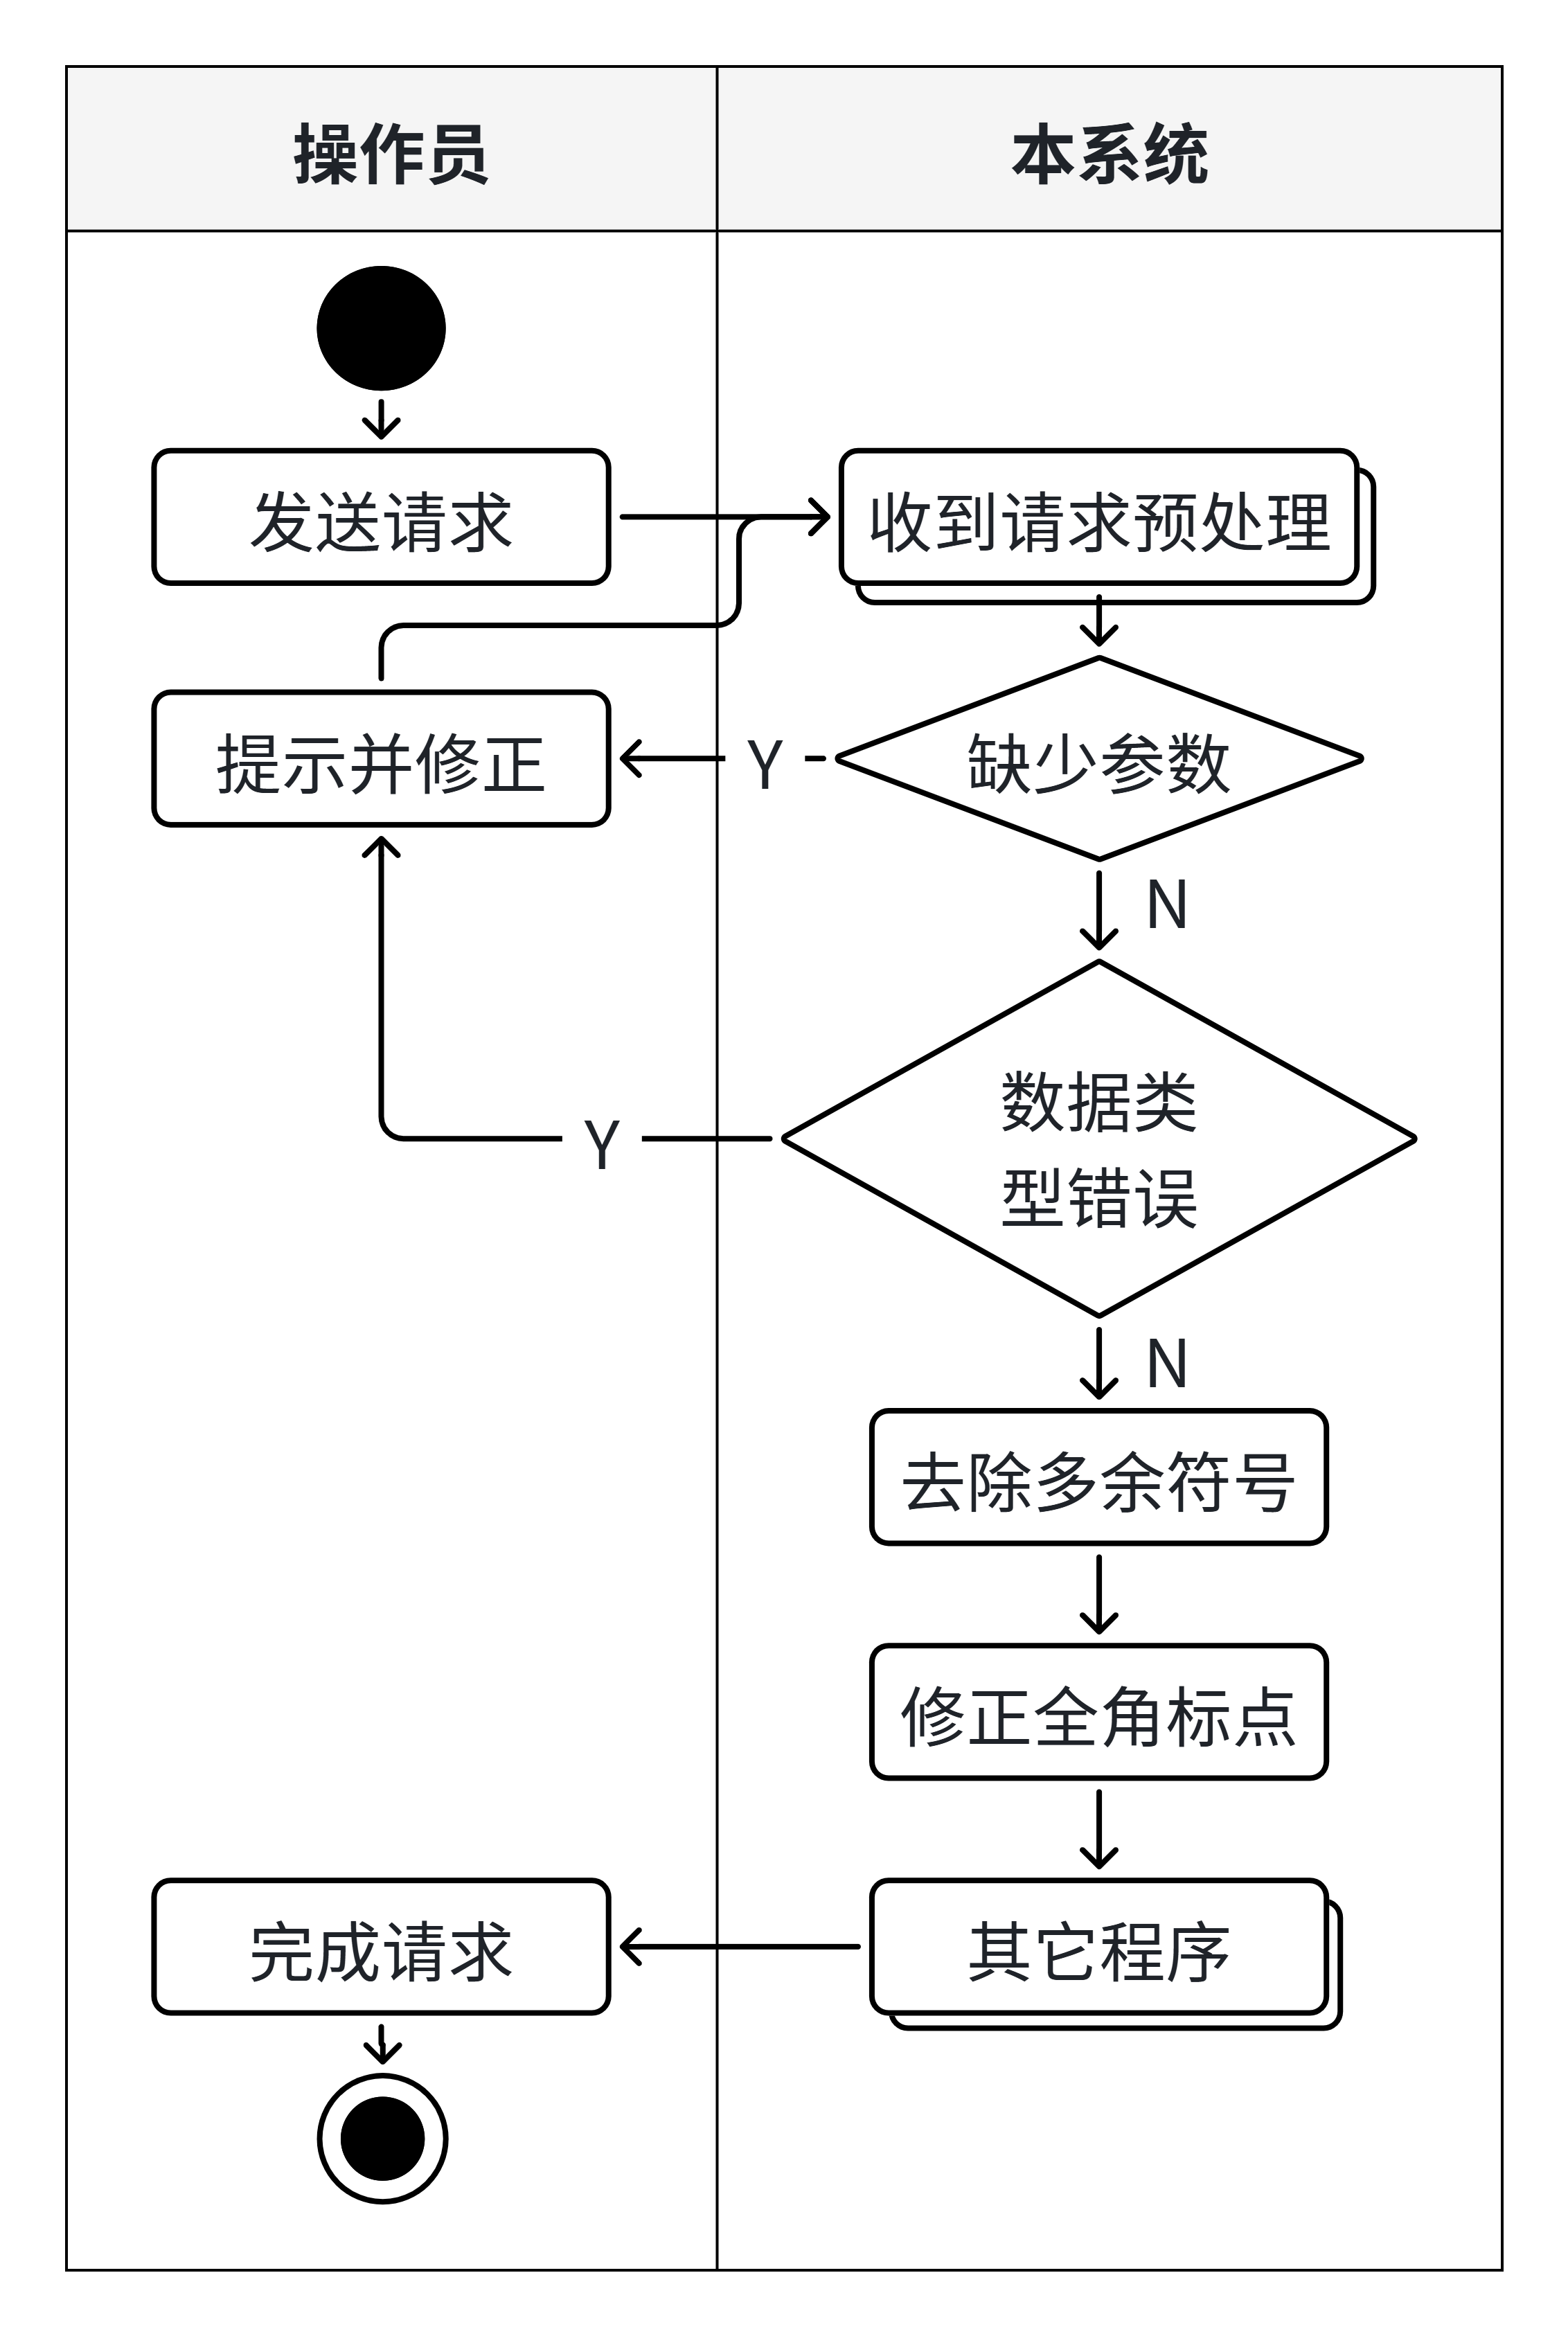
\includegraphics[width=0.8\linewidth]{figures/5/数据校验模块流程.png}
    \caption{数据校验模块泳道图}
    \label{fig:enter-label}
\end{figure}

\section{任务调度层详细设计}

本节着重介绍任务从API层提交至执行层执行前的相关过程。API层的设计较为简洁，其核心关注点在于权限验证以及数据的正确性，并不涉及对深层次需求与逻辑的处理。

当API层接收到任务后，会将任务简要地写入数据库，并将任务状态设为 “待调度”，同时把该任务添加至任务池。本系统前端网页操作员编辑任务到该任务被调度，整体的流程如图5.3所示。

\begin{figure}[htbp]
    \centering
    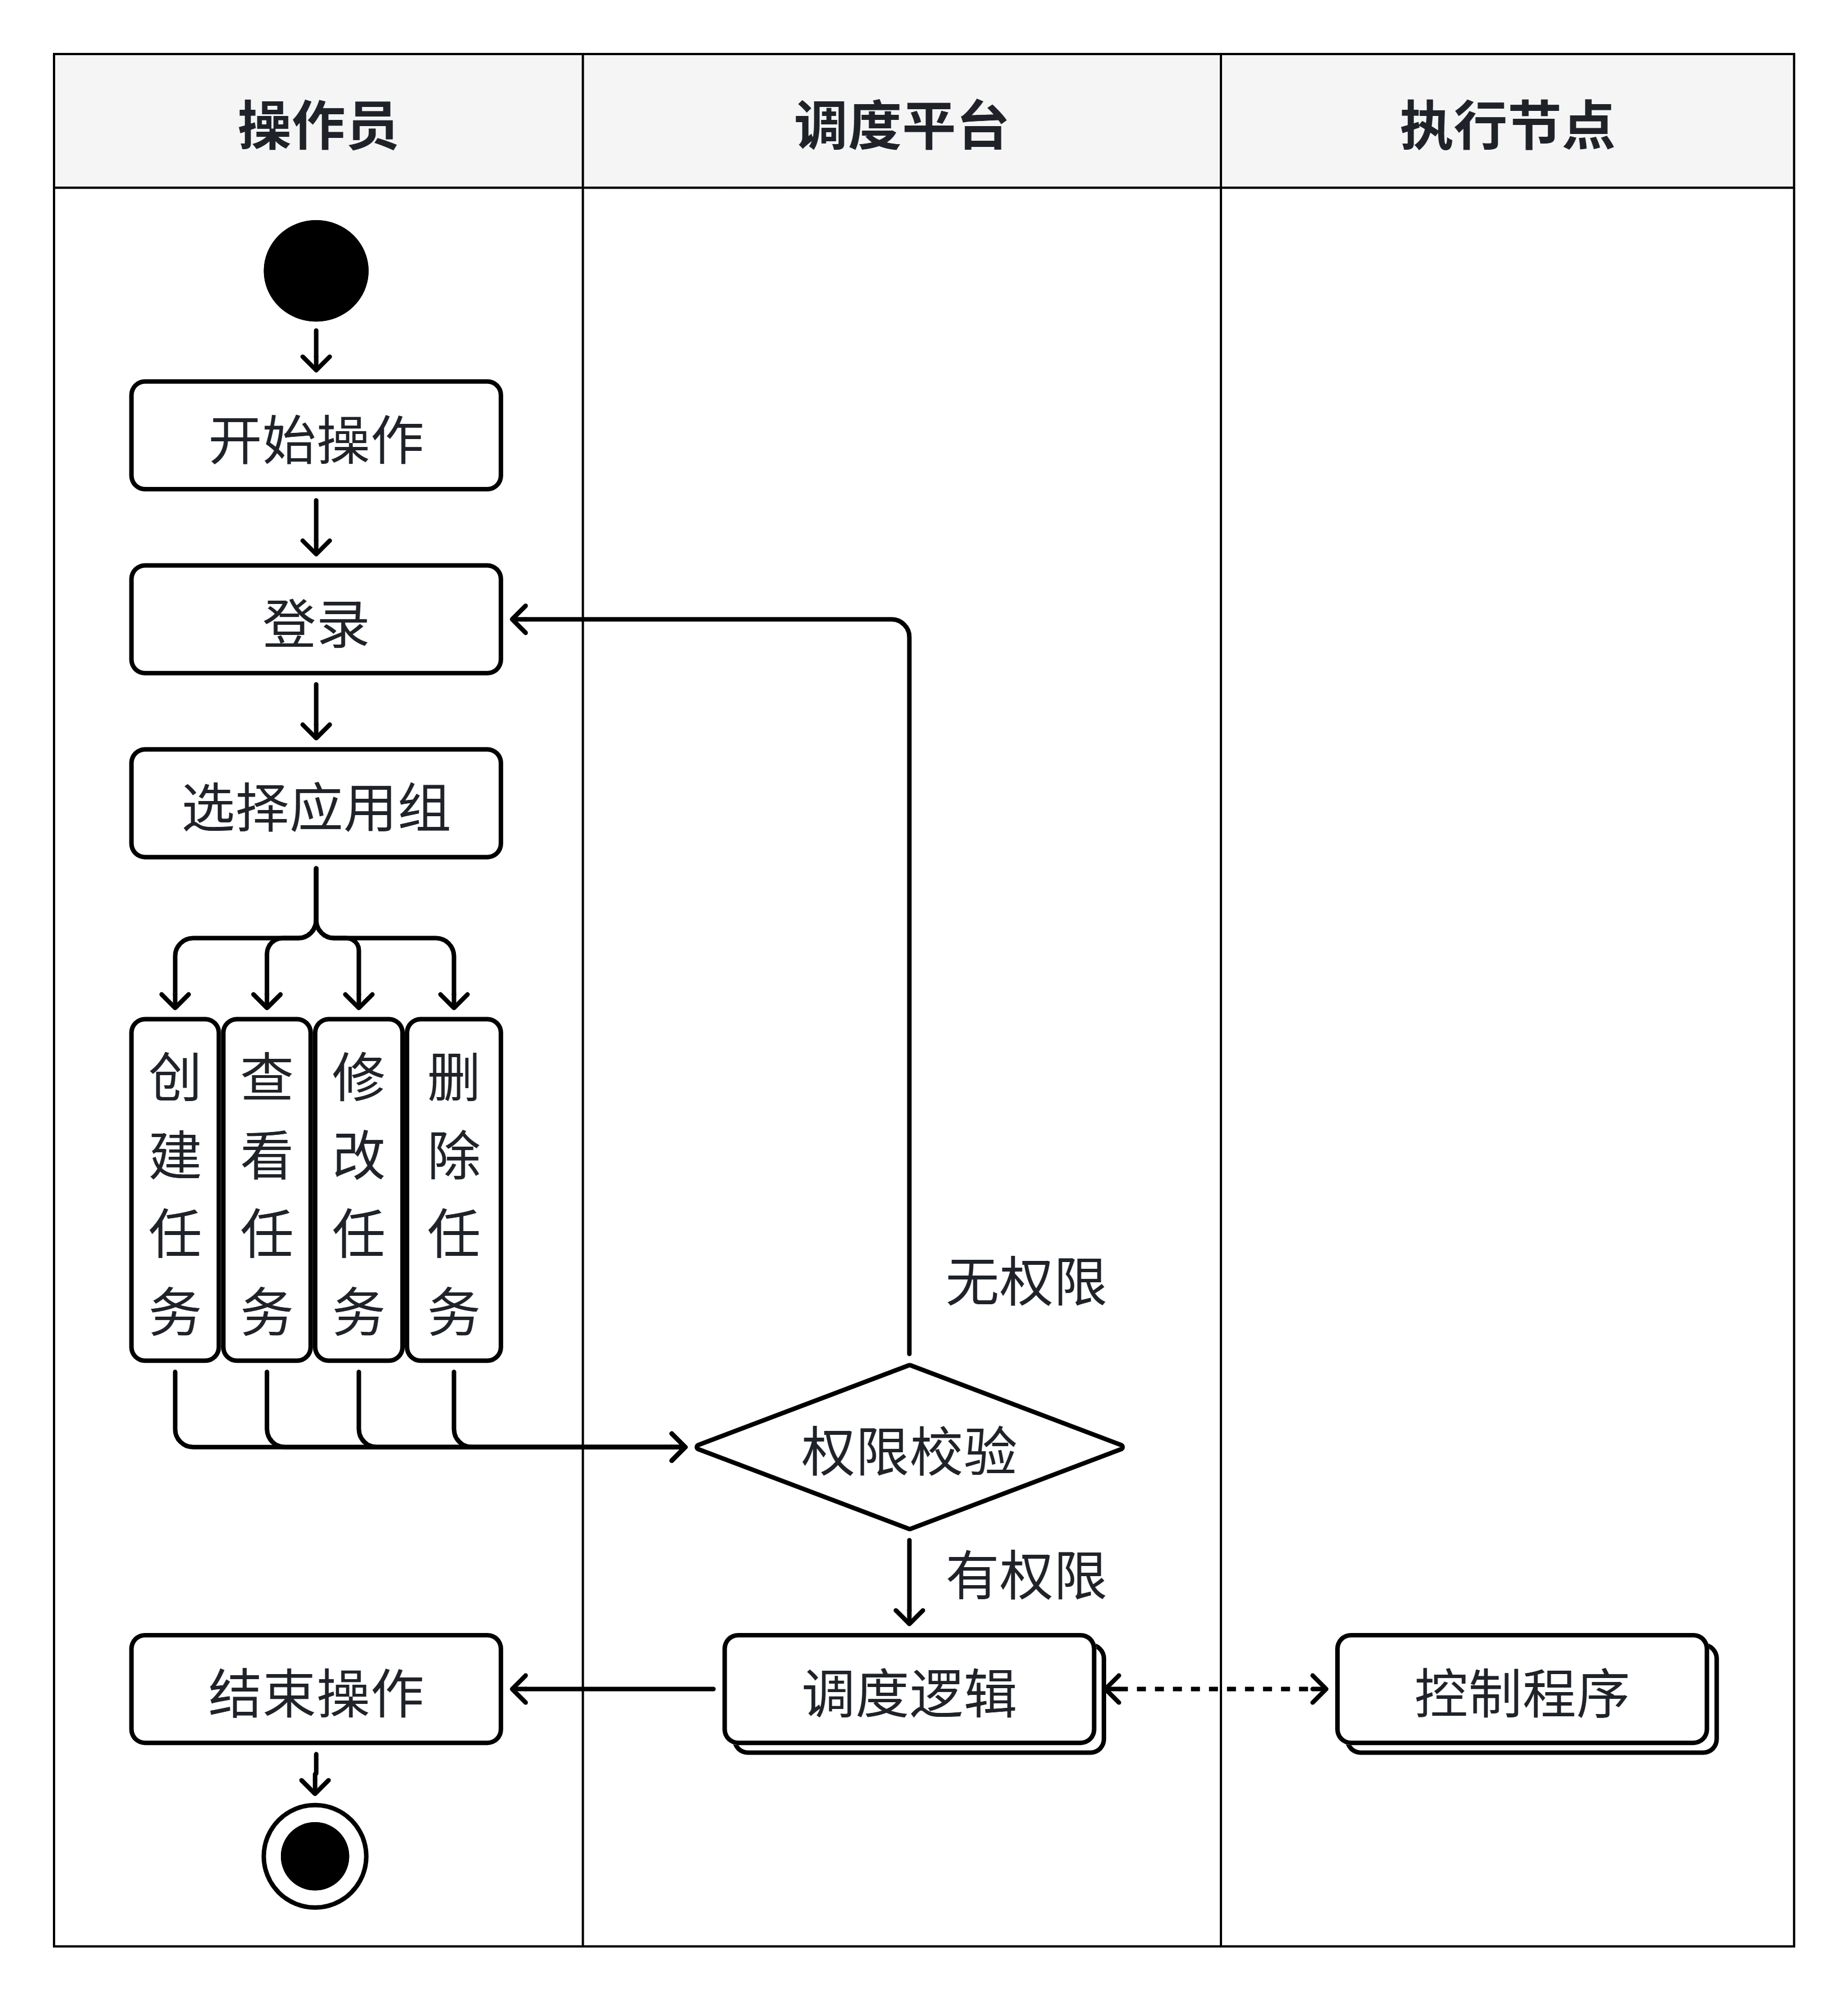
\includegraphics[width=\linewidth]{figures/5/任务操作流程图.png}
    \caption{任务操作泳道图}
    \label{fig:enter-label}
\end{figure}

本系统构建了一套任务状态管理模型，旨在实现对任务全生命周期的精细化追踪与实时监控。
该状态机不仅是调度系统的逻辑枢纽，为各模块间的协同运作提供统一的状态视图，同时也是各类调度启发式算法执行资源互斥分析与自动化准入决策的关键依据。通过状态机的统一管理与维护，系统能够准确记录任务在不同阶段的执行状况，为上层调度策略提供可靠的事实来源；
借助对任务状态的精确原子化控制，系统能够动态感知任务推进过程中的状态变化，进而优化调度序列，在保障AI多任务场景下资源分配合理性的同时，确保各项任务的有序流转与合规执行。最终，这套模型在复杂的异构计算环境中构建起一道逻辑屏障，在提升资源吞吐效能的同时，最大程度地降低了任务因状态失稳而导致的交付风险。
各状态的具体定义与语义说明如表5.1所示。

\begin{table}[htbp]
    \centering
    \caption{任务状态说明表}  % 表格标题（可按需修改）
    \begin{tabular}{lll}
        \toprule
        状态名称 & 状态含义 & 状态描述 \\
        \midrule
        WAITING  & 等待中 & API层提交后的状态，等待系统调度 \\
        SUSPEND  & 已挂起 & 经手动挂起，不会被调度 \\
        SENT     & 已调度 & 已调度并发送至执行队列 \\
        PENDING  & 等待中 & 执行队列已接收，正在队列本地等待执行 \\
        STARTED  & 已启动 & 已开始执行，但未上报进度信息 \\
        PROGRESS & 执行中 & 正在执行，并且已上报进度信息 \\
        SUCCESS  & 已成功 & 分支状态，任务已成功运行 \\
        FAILURE  & 已失败 & 分支状态，任务运行失败 \\
        REVOKED  & 已撤销 & 条件状态，任务已撤销 \\
        \bottomrule
    \end{tabular}
    \label{tab:task_status}  % 表格引用标签（可按需修改）
\end{table}

本系统通过状态机实现对AI任务全生命周期的精确原子化控制，其状态迁移逻辑可细化为三个关键阶段：

\begin{enumerate}
    \item 在准入与挂起阶段，任务于API层创建后的初始状态被设定为WAIT（等待中）。此时，调度模块会持续扫描该状态的任务，通过自动化决策引擎验证其是否同时满足业务策略限制与临界资源无冲突这两个核心前置条件，从而呼应了对自动化决策与资源互斥的研究。一旦校验通过，系统将自动触发调度指令并将状态迁移至SENT（已发送）；为保障运维灵活性，操作员可在调度前手动将任务切换至SUSPEND（已挂起）状态，使其进入逻辑隔离区并被调度算法静默忽略，直至手动恢复。
    \item 在队列排队与执行阶段，状态流转侧重于算力资源的实时分配与执行反馈，以适配AI任务的长周期特性。当任务进入执行层队列后被标记为PENDING（排队中），等待算力节点拾取并启动计算进程，随后状态迁移为STARTED（已启动）。针对AI任务耗时长且过程不透明的特点，执行层支持异步上报计算指标，接收到心跳或进度数据即转为PROGRESS（执行中），并实时映射至面板。
    \item 在任务终态与资源释放阶段，系统依据标准化接口的返回结果完成状态归档。通过捕获Python函数的布尔型返回值，系统可自动判定任务执行结果为SUCCESS（成功）或FAILURE（失败）。此外，本系统支持全局撤销指令，任务一旦被撤销，状态立即变更为REVOKED（已撤销）。处于该状态的任务将强制触发临界资源的释放逻辑，并不再参与后续的任何调度计算。
\end{enumerate}

整体状态机迁移逻辑与分布式异步协作时序分别如图5.4和图5.5所示。

\begin{figure}[htbp]
    \centering
    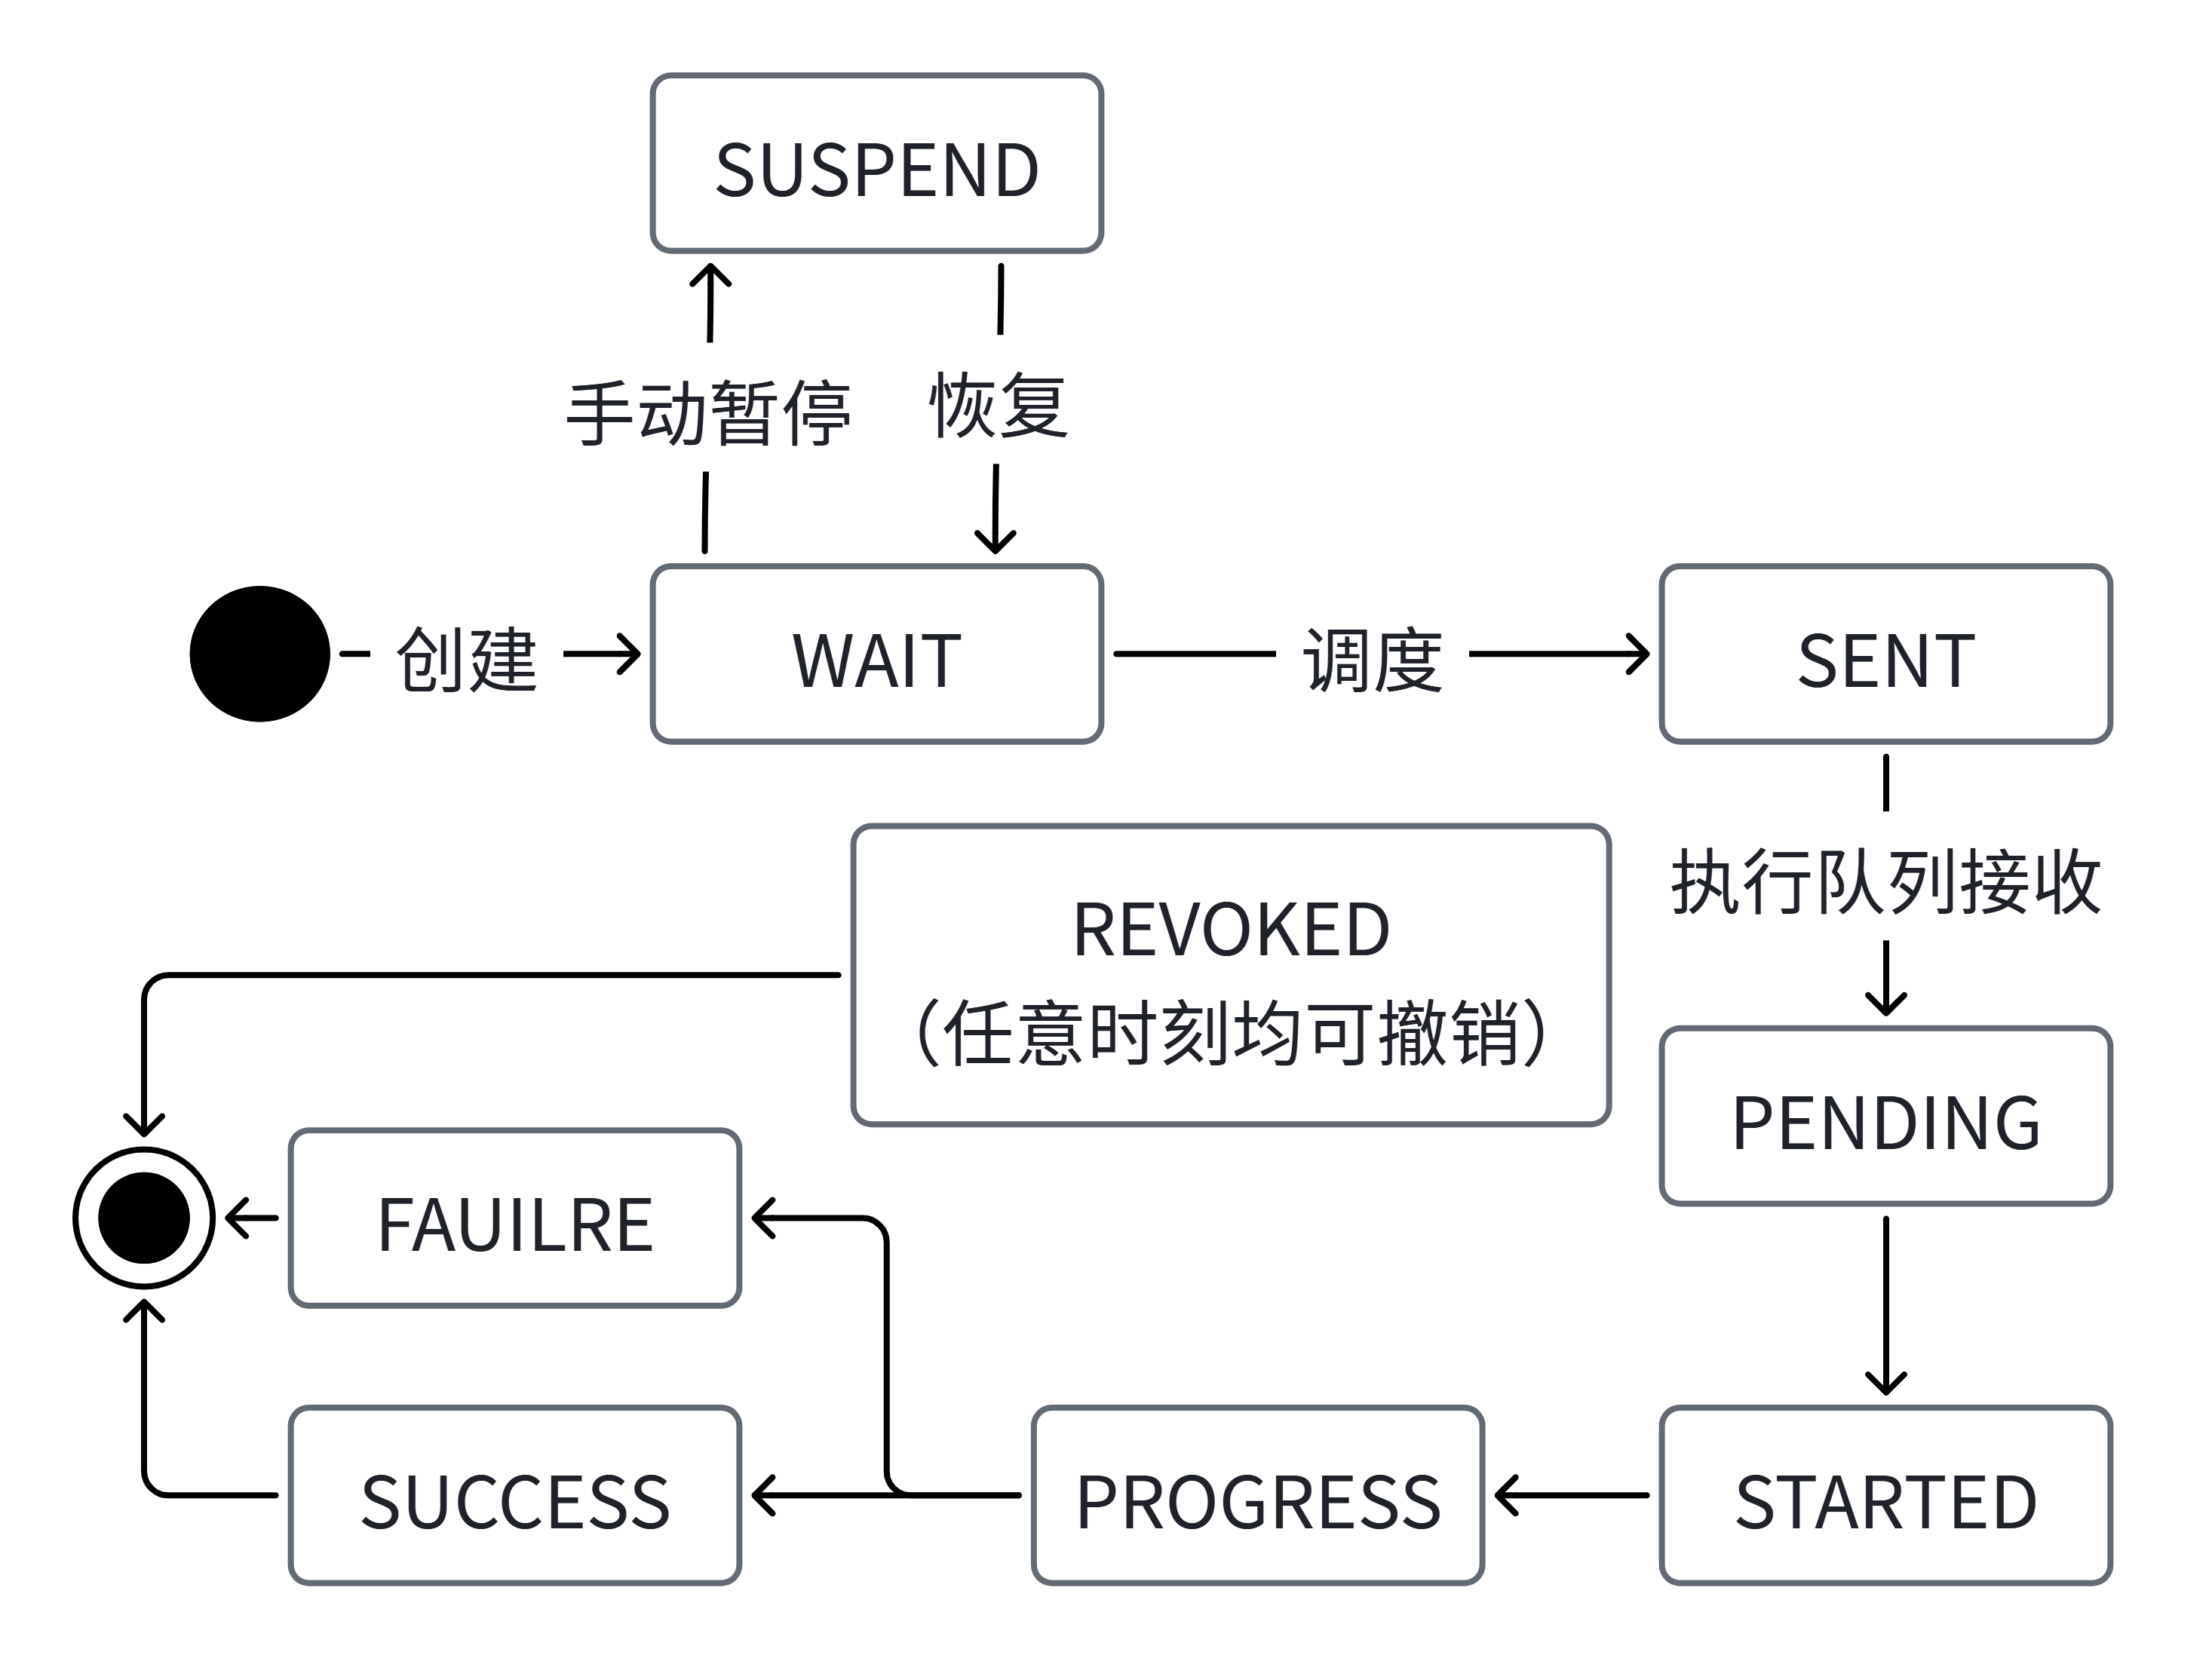
\includegraphics[width=0.8\linewidth]{figures/5/任务状态机.png}
    \caption{任务状态机}
    \label{fig:enter-label}
\end{figure}

\begin{figure}[htbp]
    \centering
    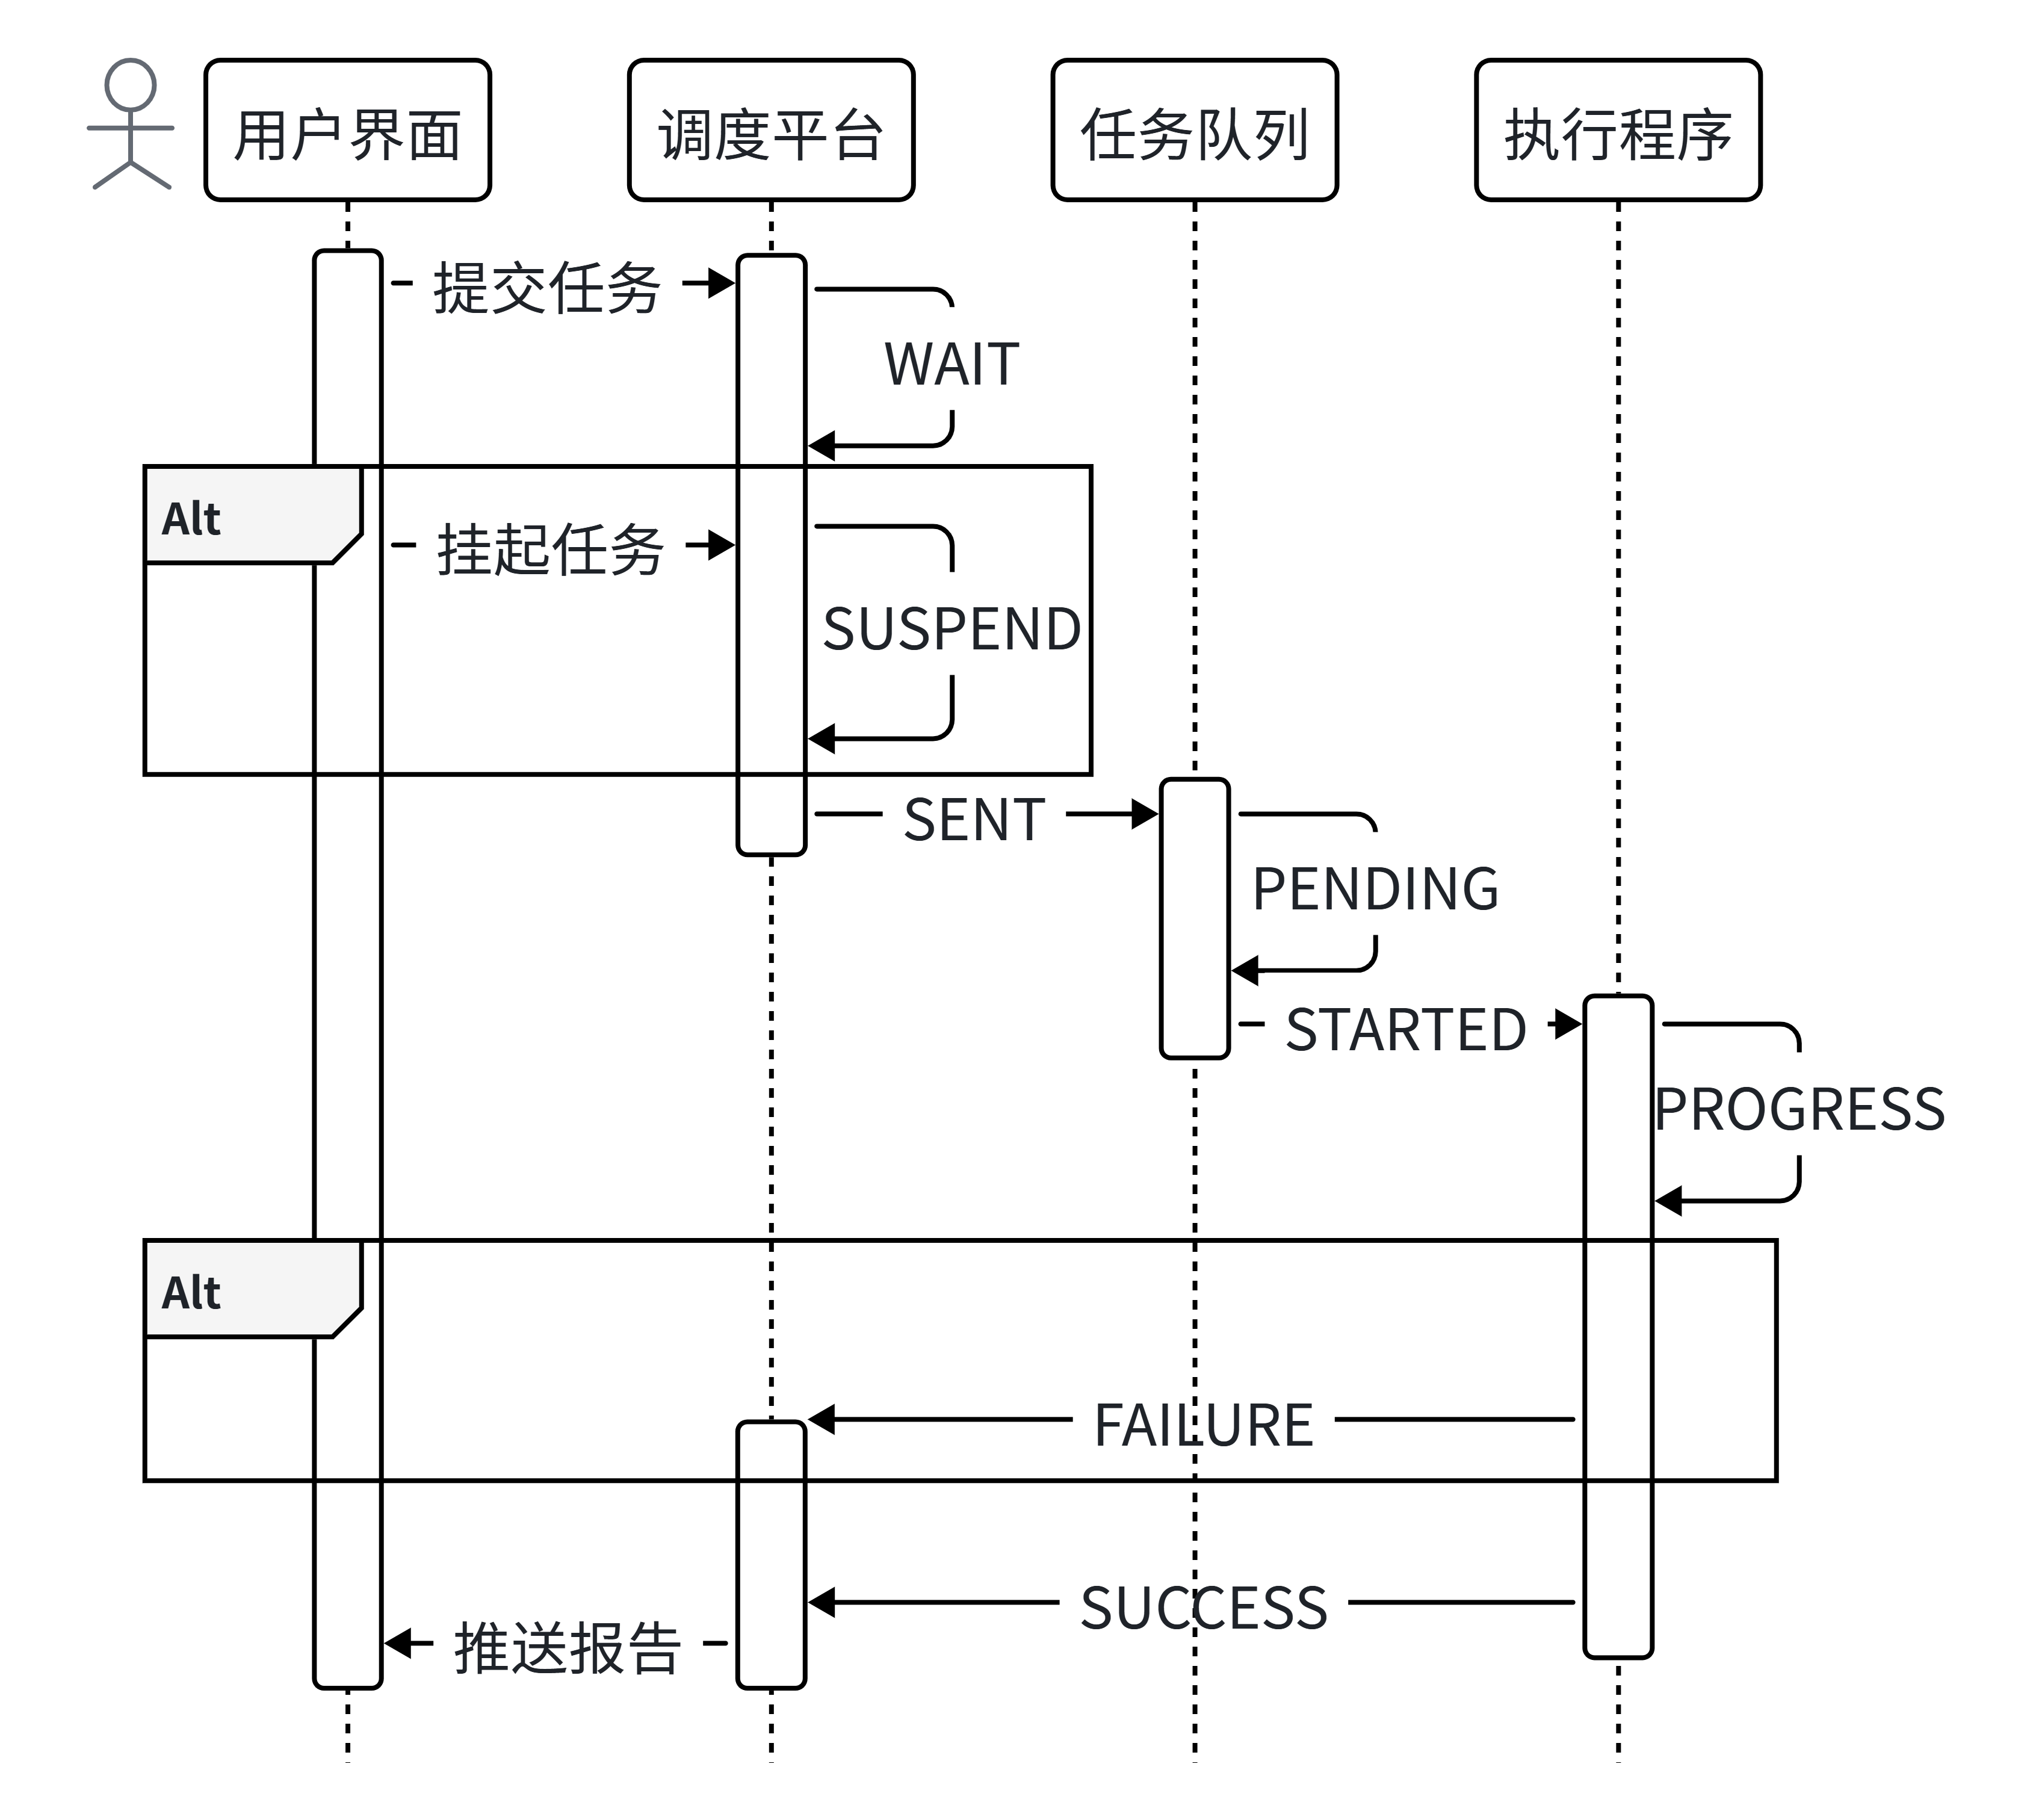
\includegraphics[width=0.8\linewidth]{figures/5/状态机时序图.png}
    \caption{状态机时序图}
    \label{fig:enter-label}
\end{figure}

\subsection{任务可用性检测}

本机制的设计与实现旨在攻克调度决策过度依赖人工判断的瓶颈。其研发过程经历了由静态硬编码向动态配置化逻辑引擎的演进：初期方案由于需求边界模糊，采用硬编码方式实现逻辑判断，缺乏灵活性；随着研究深入，本系统通过对多维业务场景进行需求调研与特征提取，构建了基于配置驱动的通用逻辑引擎。该设计允许管理员在不触动核心代码的前提下，通过修订策略配置文件即可实现调度逻辑的快速更迭。

任务可用性检测的核心在于构建一套具备环境感知能力的自动化决策体系。系统在调度周期内自动采集任务优先级、实时资源占用、环境兼容性等前置参数，并联动动态加载的策略规则进行多维度校验，最终自主输出“即时执行”或“挂队等待”的准入指令。从工程架构上看，逻辑引擎采用“解析-缓存-判定”的流水线模式。系统初始化阶段预先加载JSON格式的策略文件并将其序列化至内存规则库，在接收到调度请求时，引擎按“环境指标采集-策略规则匹配-准入结果判定”的逻辑链条执行自动化比对。这种配置驱动的架构设计，显著提升了系统在高动态AI研发环境下的扩展性与运维响应速度。

为实现复杂业务逻辑的标准化表达，本系统抽象出“条件”与“规则”两大核心算子。条件（Condition）： 逻辑判定的最小原子单元，用于评估特定环境下状态的真伪。每个条件由“编码（Code）”、“判断参数（Params）”及“固化逻辑”组成。其映射关系可表示为：
$$C = \{Code, Params\} \rightarrow f_{logic}(Env, Params)$$
其中，$Code$唯一标识底层判断逻辑，$Params$（如起始时间、负载阈值）则赋予同一逻辑适配不同场景的灵活性。规则（Rule）： 由原子条件经逻辑算子嵌套组合而成的复合表达式。本系统采用二级嵌套结构实现复杂的调度策略：一级数组元素间执行“或（OR）”逻辑，二级数组元素间执行“且（AND）”逻辑。其逻辑范式如下：
$$Rule = \bigvee_{i=1}^{n} \left( \bigwedge_{j=1}^{m} Condition_{i,j} \right)$$
这种结构支持高度灵活的策略表达，从而实现对异构任务的差异化准入控制。

针对多任务场景下的动态需求，系统建立了“任务-场景”双维度关联机制。每个任务类型绑定唯一任务编码及默认规则簇，而场景策略具备更高的决策优先级。调度引擎执行时，优先检索当前环境特征对应的场景规则。若场景规则命中，则优先执行场景约束；若无场景匹配，则回退至通用任务规则。这种优先级覆盖的机制，确保系统在节假日、算力峰值等特殊时空节点下，能够通过场景策略的实时注入，精准实现对AI多任务的智能流量分摊与风险规避。

任务可用性检测机制逻辑引擎的总体结构如图5.6所示。

\begin{figure}[htbp]
    \centering
    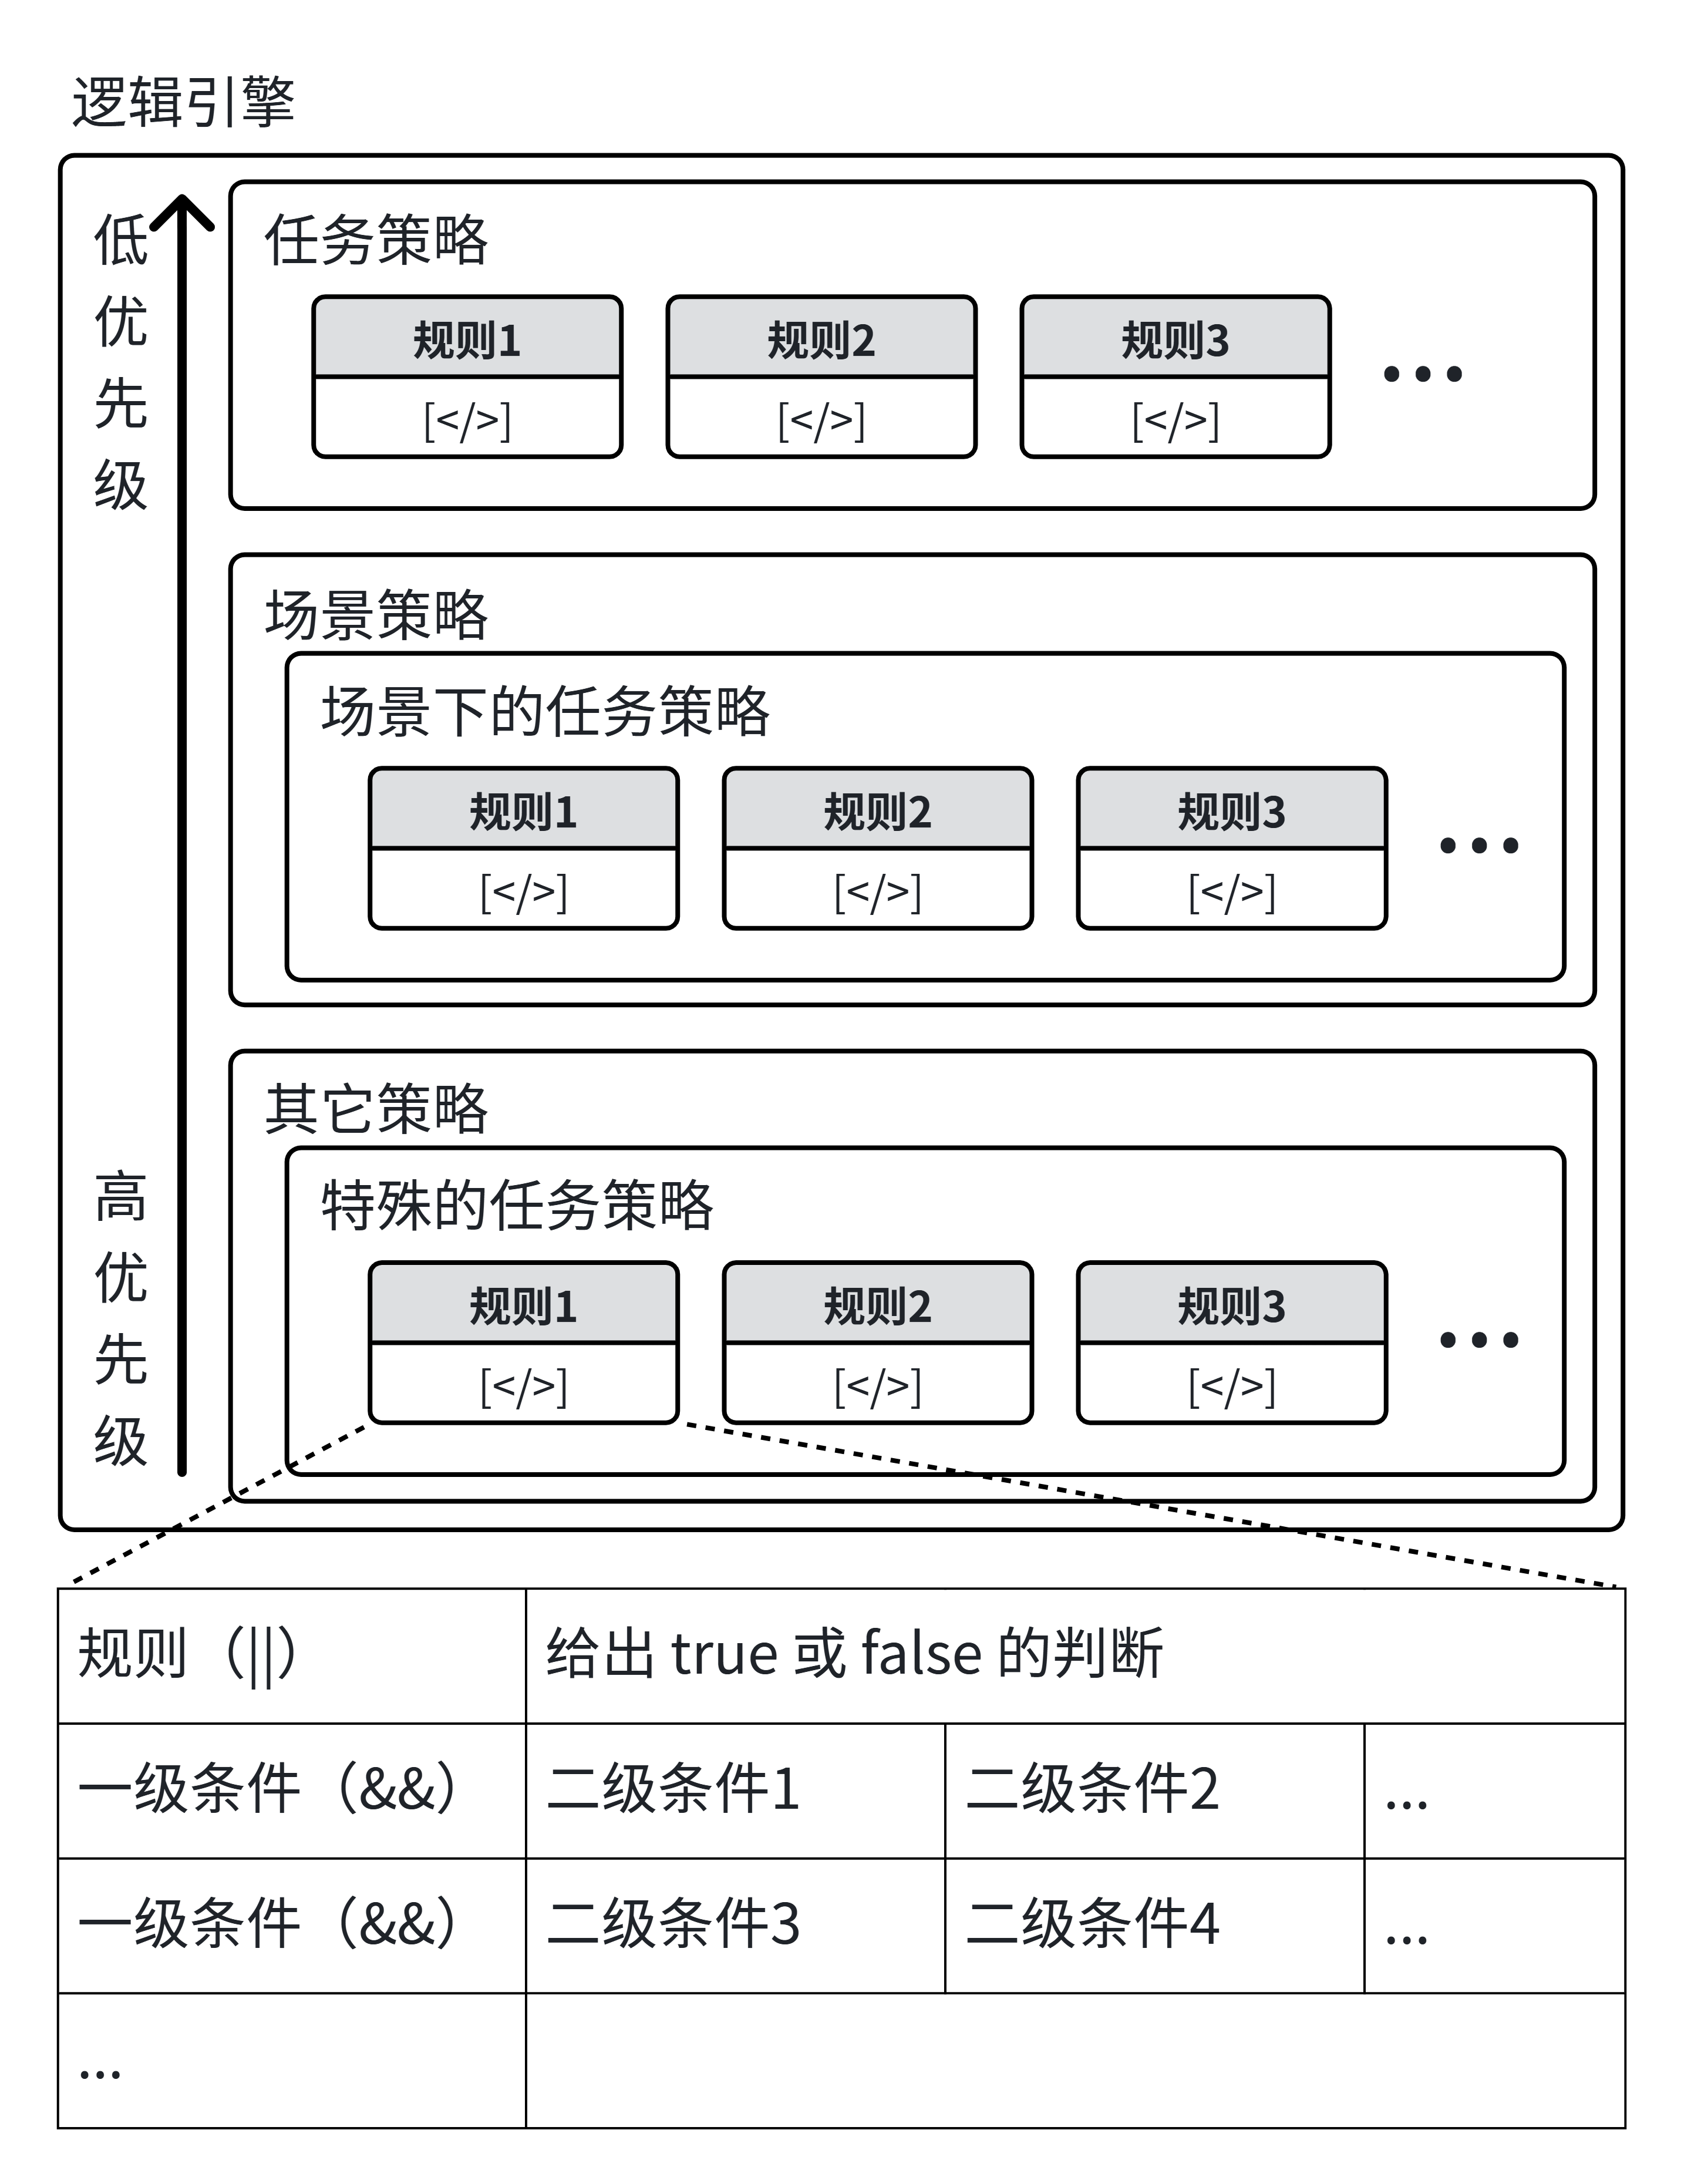
\includegraphics[width=\linewidth]{figures/5/逻辑引擎总体结构.png}
    \caption{逻辑引擎总体结构}
    \label{fig:enter-label}
\end{figure}

\subsection{资源可用性检测}

本机制的核心目标是解决子问题三中提到的“缺乏资源互斥智能分析能力导致的计算资源浪费”难题。在人工智能多任务场景下，GPU等算力资源通常具有强独占性。若调度算法无法精准识别不同任务间的资源依赖冲突，强行并发执行会导致显存溢出或计算数据冲突，进而造成任务失败与算力资源的严重空耗。因此，本机制通过构建细粒度的资源拓扑识别逻辑，实现了由“保守串行调度”向“高效并发调度”的转型。

从工程演进路径来看，资源可用性检测机制是系统实现“算力精细化治理”的关键跃迁。在系统研发初期，为保障核心框架的快速上线，调度逻辑侧重于基础任务流转；而在后续的迭代过程中，本系统通过三个版本的深度演进，逐步引入了动态资源锁机制与异步释放逻辑，使其能够灵活适配复杂异构场景下的临界资源约束。

\begin{table}[htbp]
    \centering
    \caption{资源占用表}
    \begin{tabular}{llllll}
        \toprule
        序号 & 字段名 & 字段说明 & 类型 & 是否可选 & 说明 \\
        \midrule
1 & task\_id & 任务ID & int & N &  \\
2 & resource\_id & 资源ID & int & N &  \\
3 & is\_delete & 此条记录是否有效 & boolean & N &  \\
4 & id & 本条记录id & int & N &  \\
        \bottomrule
    \end{tabular}
    \label{tab:my_label}
\end{table}

为支撑高效的互斥判定，系统建立了如表5.2所示的资源占用记录表。该表作为全局调度状态的“实时快照”，通过简洁的三元结构实现了任务与临界资源的高性能映射。该模型的设计逻辑在于：通过 task\_id 与业务任务表建立多对一关联，实现对单一任务多维度资源依赖的完整覆盖；利用 is\_delete 字段实施状态柔性管理，在任务撤销或异常终止时，系统通过逻辑删除实现算力资源的秒级释放，无需物理删除历史记录，既提升了数据库吞吐量，又为后续的算力使用审计提供了全量数据溯源支持。

资源可用性检测的操作逻辑通过“静态注册-动态探测-准入控制”的闭环流程，实现了对AI临界资源的精细化治理，从技术底层化解了算力冲突难题：

\begin{enumerate}
    \item 资源注册：任务编写者需根据AI算子的具体执行特征（如是否涉及独占性GPU显存、特定硬件加速器等），在任务定义阶段预先声明其所需的临界资源清单。这一步骤通过元数据建模，将抽象的任务需求转化为系统可感知的资源需求矩阵，为后续的互斥分析提供了静态参考基准。
    \item 状态探测：调度引擎在触发任务下发逻辑前，会执行原子化的探测操作，实时扫描数据库中的资源占用表。系统通过检索目标资源对应的 is\_delete 标识位，判定该资源是否处于“逻辑锁定”状态。若探测到目标资源已被其他活跃任务占用，系统将精准识别此次调度动作为“互斥冲突”，并记录冲突拓扑以备后续调度参考。
    \item 并发决策：针对识别出的互斥任务，系统采取非阻塞式的“延迟重试”策略，将其自动挂起至高可靠等待队列，避免了暴力重试引发的算力波动。而对于经探测判定为资源相互独立的任务，调度引擎则打破传统的串行执行模式，在验证任务可用性后立即触发并发执行。这种基于资源感知的动态分流机制，极大缩短了任务间的间隙空耗，显著提升了异构计算集群的整体吞吐性能。
\end{enumerate}

这种基于细粒度资源感知的设计，有效打破了传统系统中由于调度盲区导致的串行执行瓶颈，最大化了多任务环境下的系统吞吐量。具体的互斥判断机制流程如图5.7所示。

\begin{figure}[htbp]
    \centering
    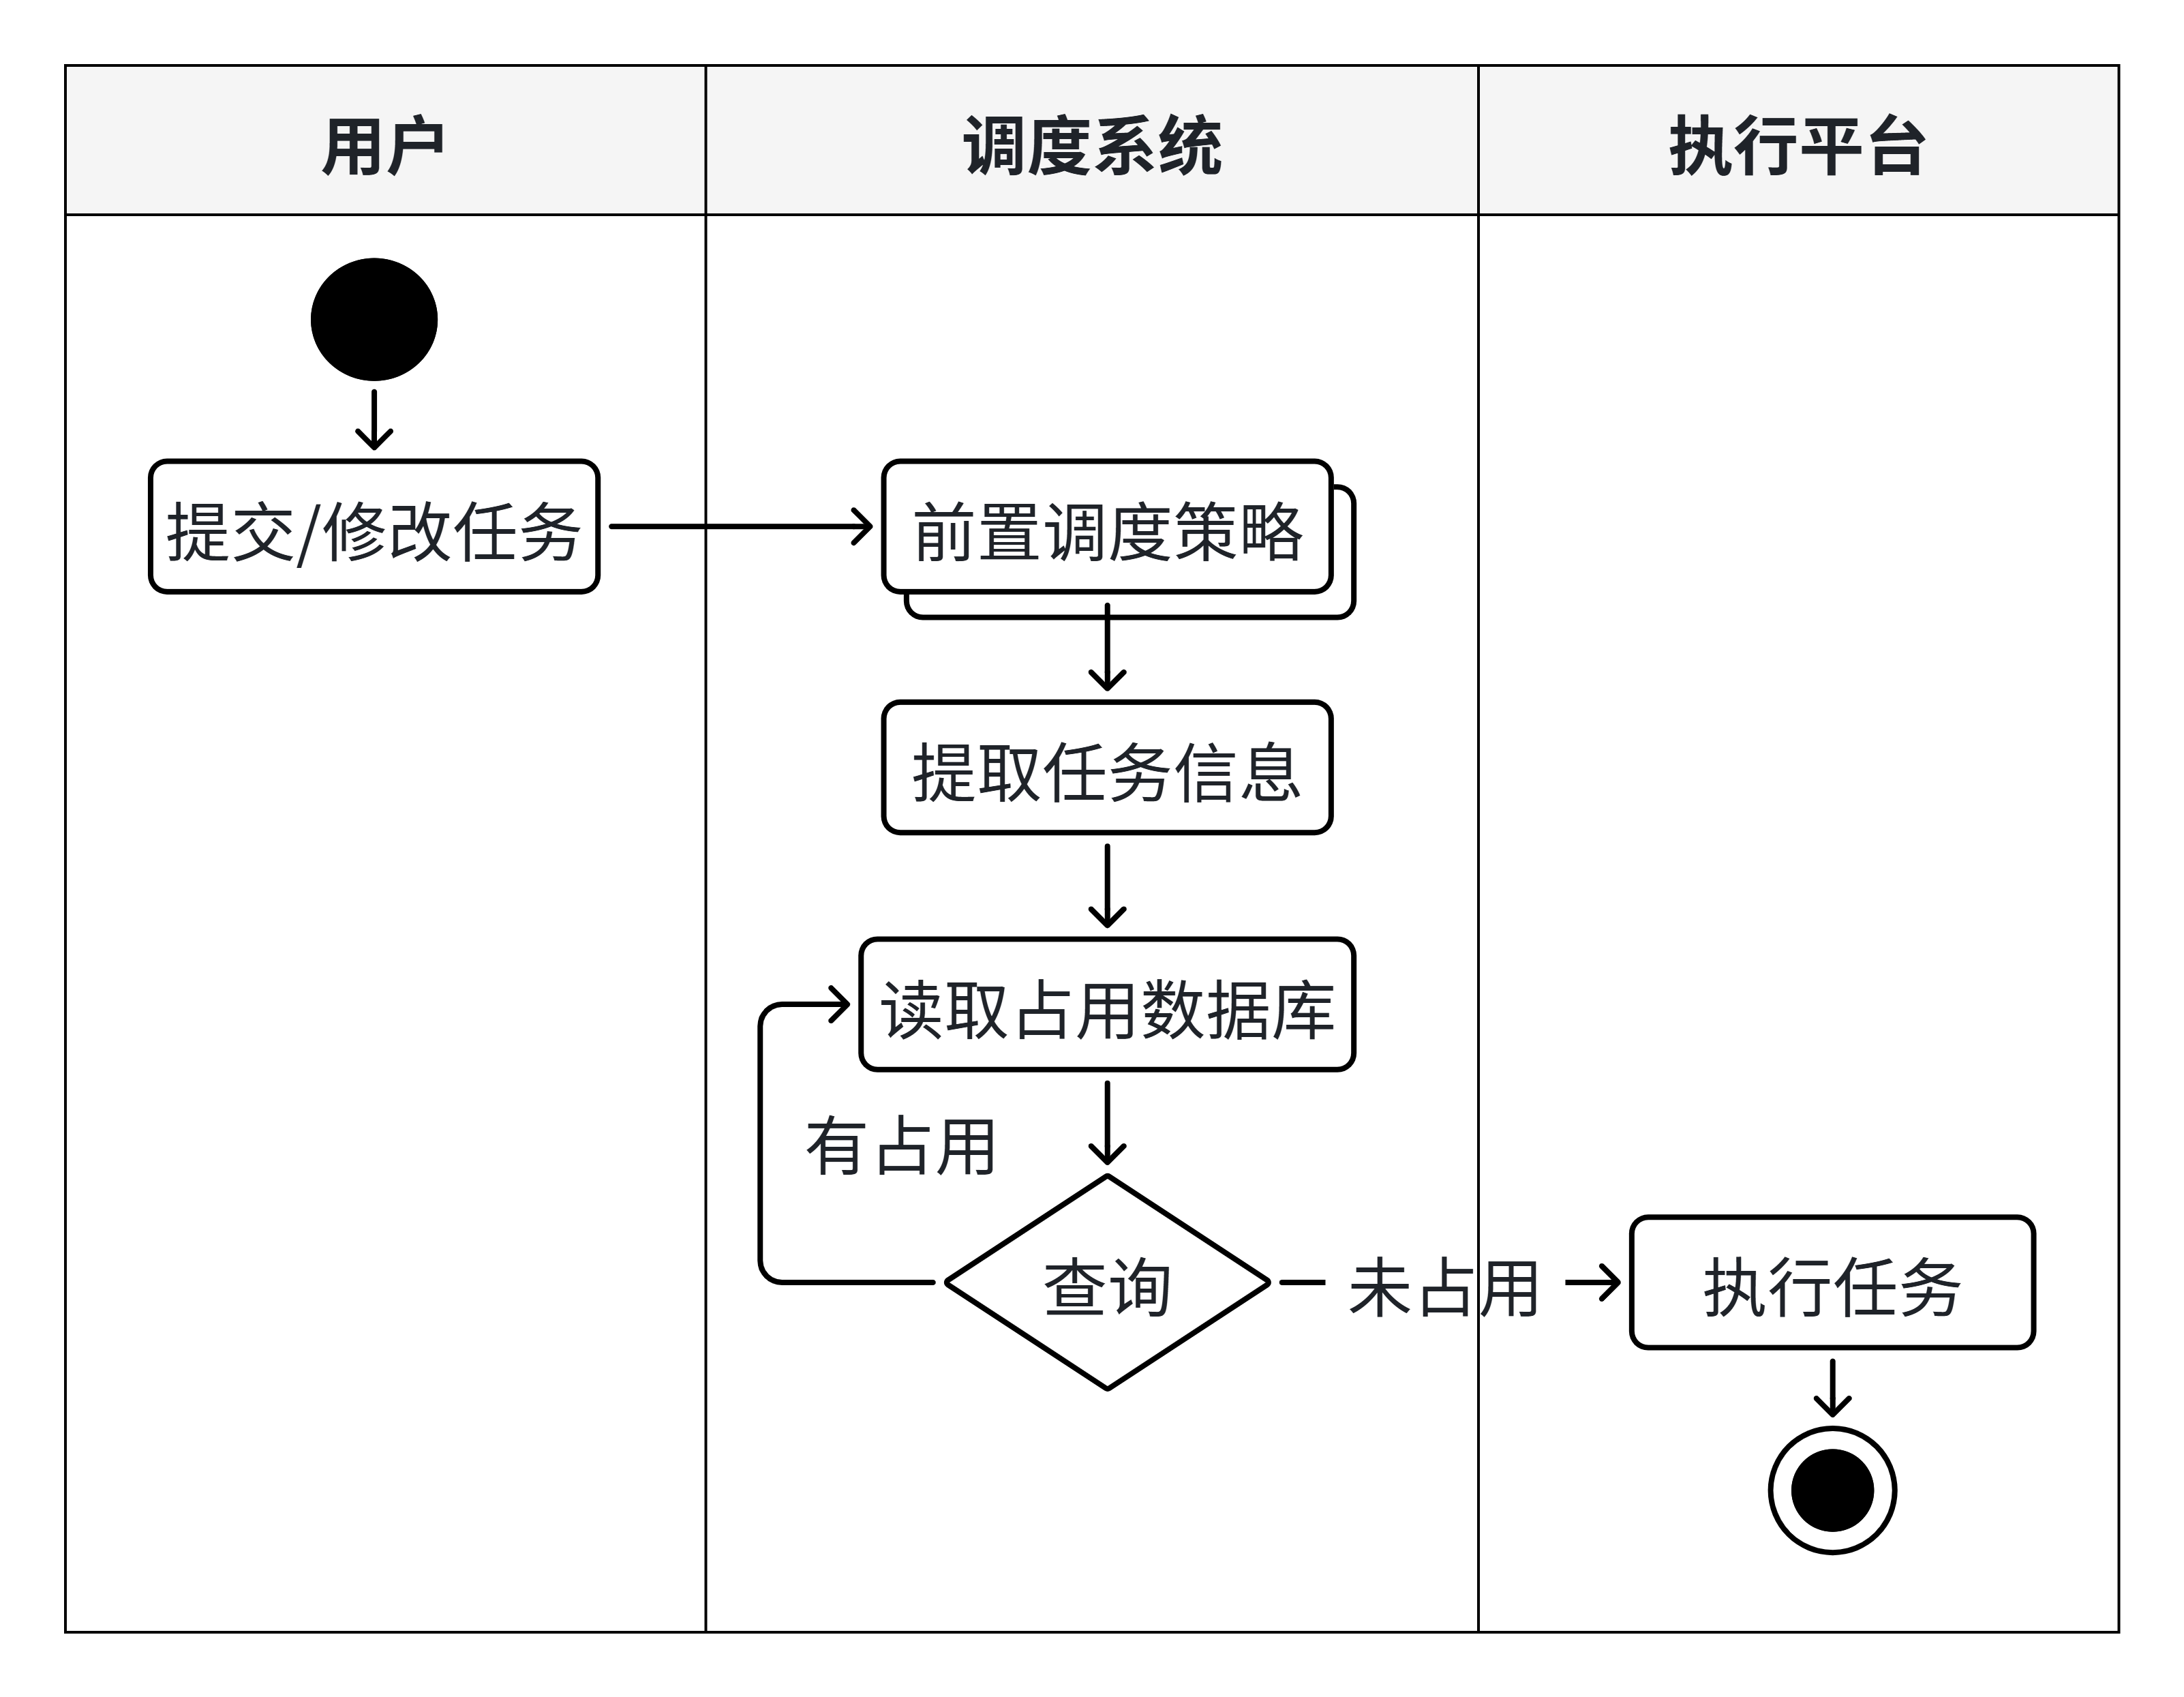
\includegraphics[width=\linewidth]{figures/5/资源互斥判断机制.png}
    \caption{资源互斥判断机制泳道图}
    \label{fig:enter-label}
\end{figure}

资源互斥判断机制，作为核心算法的一部分，与任务可用性检测互相配合，共同保障本系统的资源分配、任务运行、数据流转的正确性。

\subsection{负载均衡及性能优化设计}

本系统部署于公司内部，架构包含中心调度程序以及任务执行节点。鉴于不同开发组在预算与需求方面存在差异，其配备的任务执行节点在性能与容量上也会有所不同，因此无法采用统一的调度策略对这些节点进行管理。

在考虑云计算时，负载均衡方法的核心在于在不同的虚拟机之间分配工作负载\cite{gudivada2025}。NGINX作为业内极具领先地位的高性能HTTP服务器，其内部搭载了性能卓越的权重轮询算法，可以将请求分散到体系内的多个虚拟机上，实现了出色的负载均衡\cite{nikishin2022}。该算法凭借出色表现，在众多公司及多个领域获得了广泛应用与高度信赖。鉴于此，本系统的负载均衡算法在一定程度上借鉴了NGINX的Weighted Round Robin算法，实际上是该算法的一个简化版本。

节点通过类型与权重进行注册：类型决定任务匹配，权重表征执行能力。同一类型的节点组成“本地列表”，系统通过加权轮询算法进行调度。在单次轮询中，系统会根据权重值n在该节点连续分配n次任务后切换。该机制确保了节点的高效负载均衡，且管理员可通过将权重设为 0 实现节点的逻辑禁用。其原理如图 5.8 所示。

\begin{figure}[htbp]
    \centering
    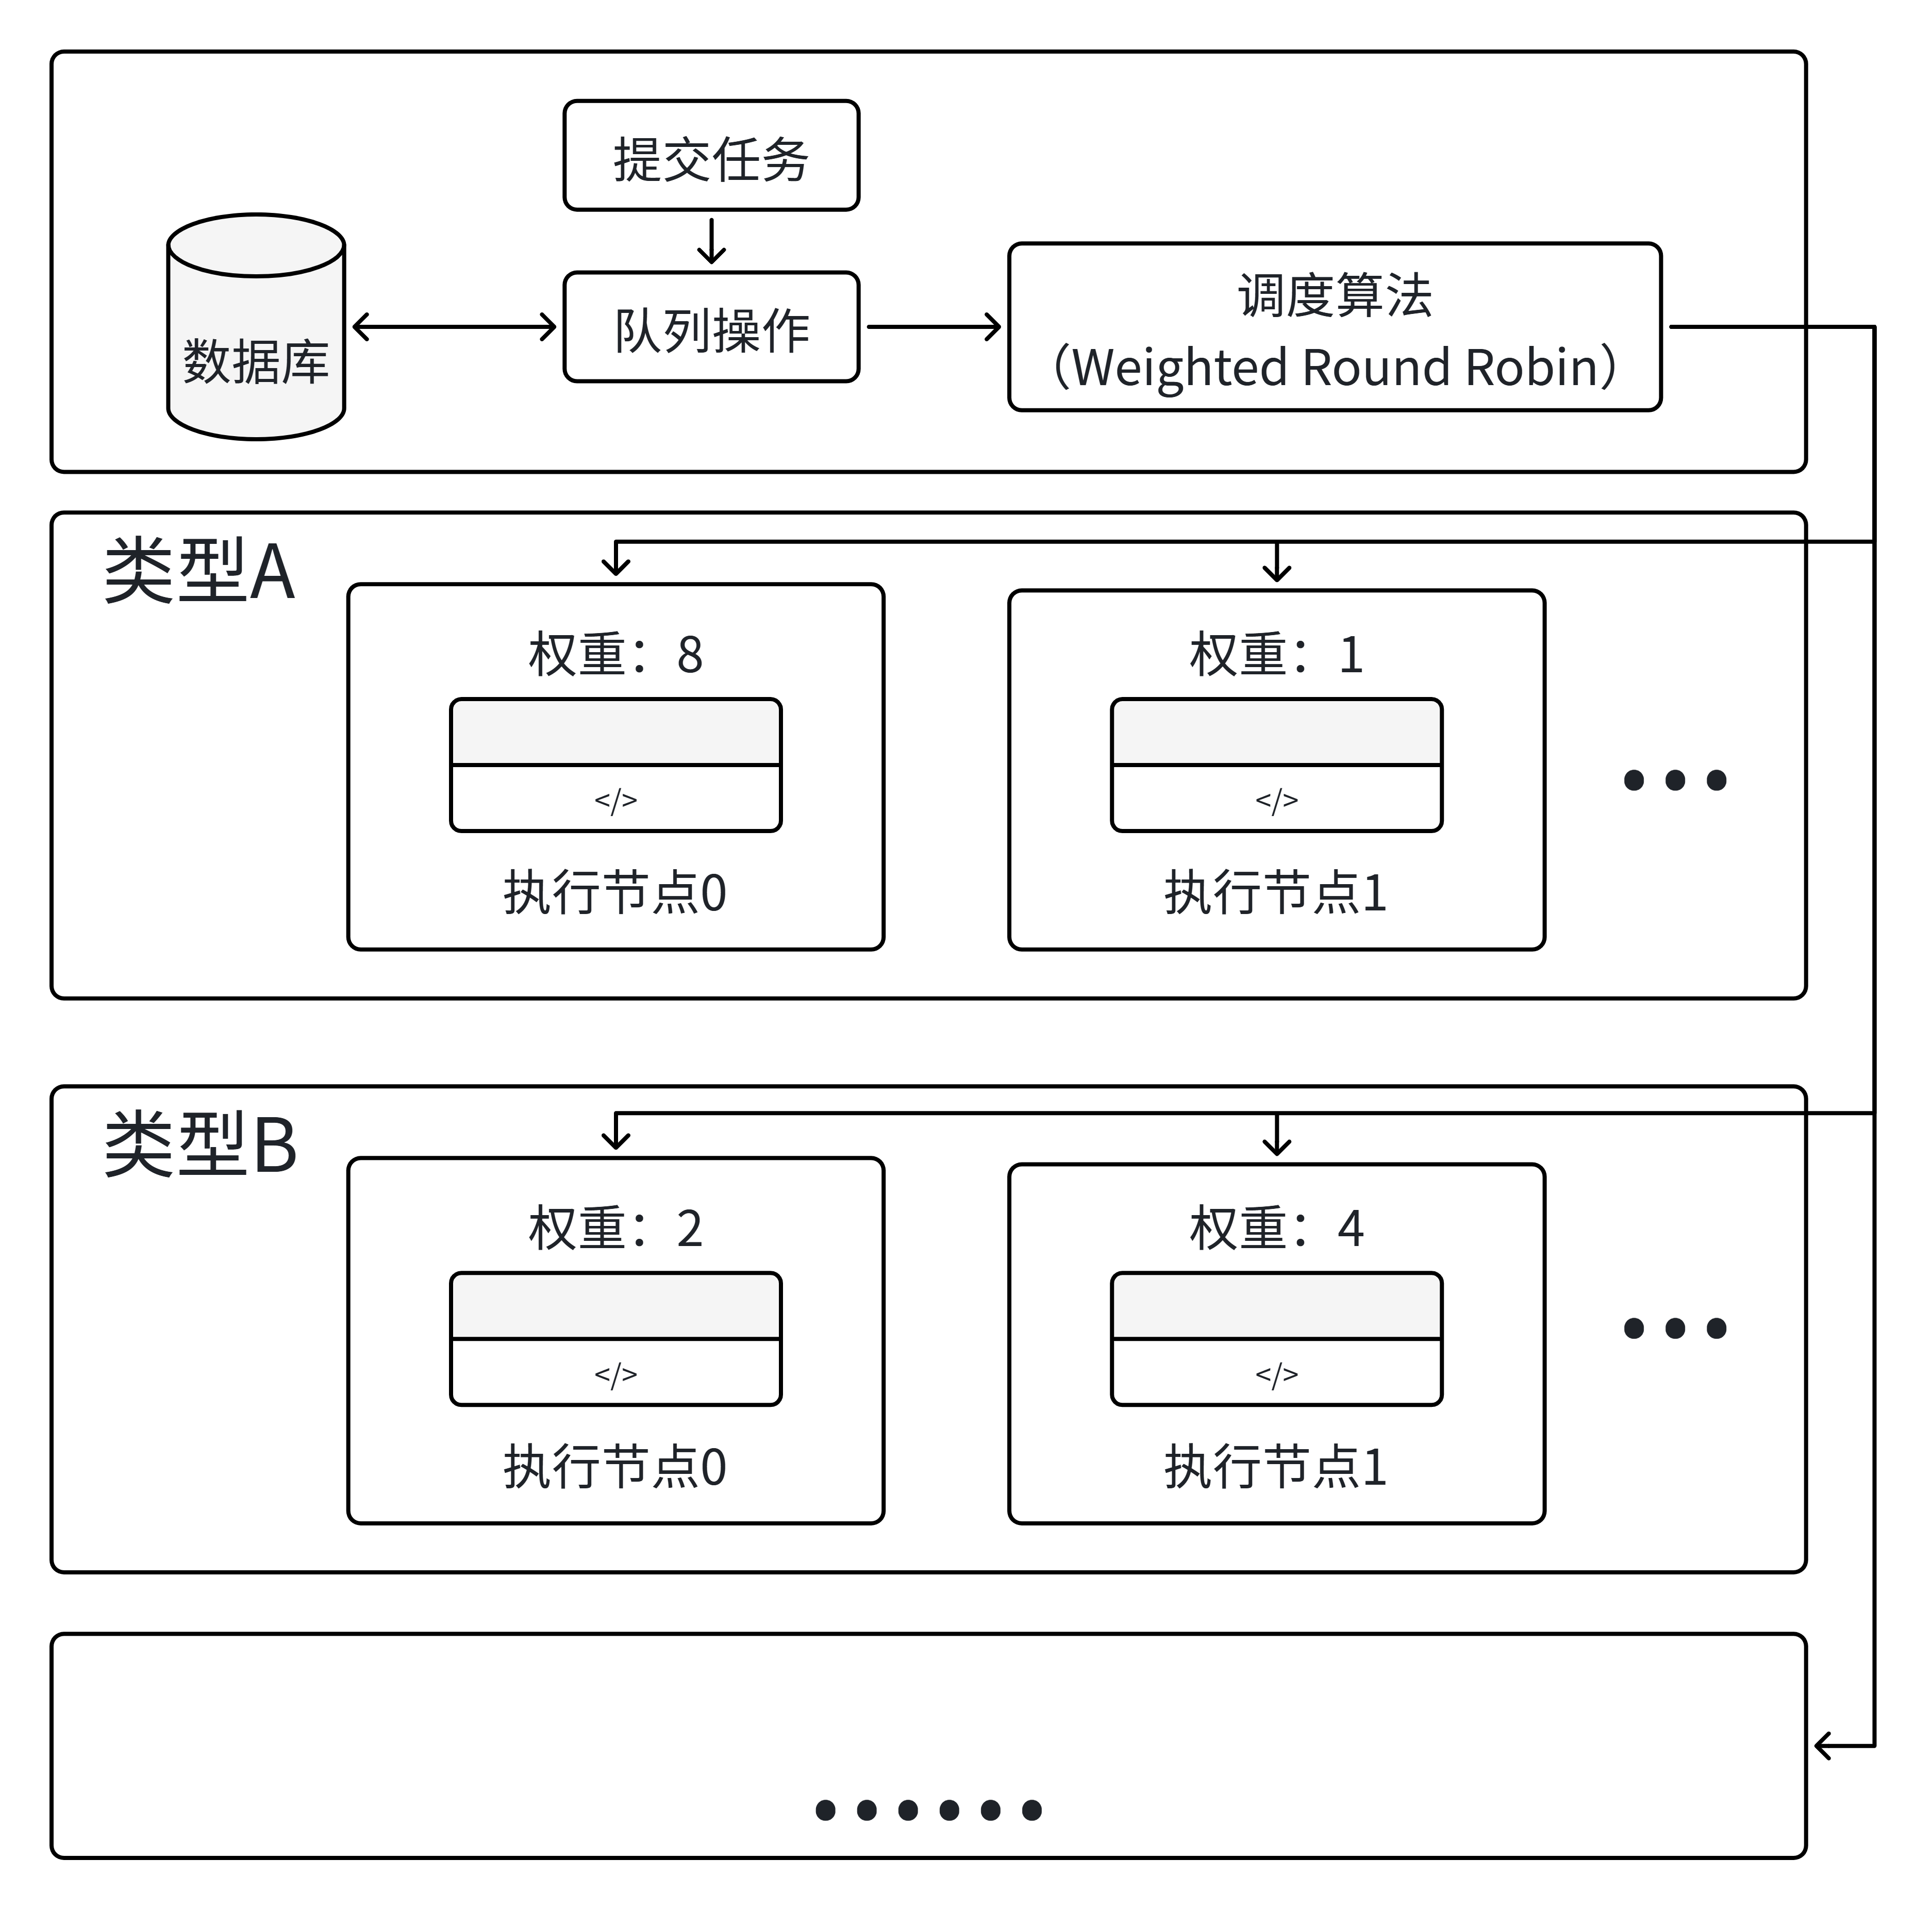
\includegraphics[width=\linewidth]{figures/5/负载均衡示意图.png}
    \caption{负载均衡原理图}
    \label{fig:enter-label}
\end{figure}

\subsection{数据同步模块}

本系统采用分布式微服务架构，由多个执行节点共同提供算力支撑。针对多模块环境下信息交互易冲突、协同效率低的痛点，系统专门设计了一套高可靠的数据同步机制。该机制通过标准化的通信链路，实现了AI任务参数与状态数据的透明流转，确保调度指令能精准下发、执行进度能实时回收，为系统实现自动化决策和资源精细化管控提供了关键的数据纽带。

在技术落地层面，系统选用Redis作为核心消息中间件，并依托Celery分布式框架实现任务的异步解耦。任务调度层会将校验纠错后的AI任务及其异构参数封装并存入Redis任务队列；执行节点作为客户端实时监听并领用任务，解析Prompt、资源列表等关键参数后，调用本地算子开展计算。任务执行完毕，节点会通过Celery将结果写回Redis。调度中枢捕获状态变更后，会即时更新本地数据库并反馈至前端，确保操作员能实时监测任务的运行状态与资源占用，彻底解决了过去由于信息流转不畅、过度依赖人工介入导致的系统效率低下问题。

数据同步模块的原理如图5.9所示。

\begin{figure}[htbp]
    \centering
    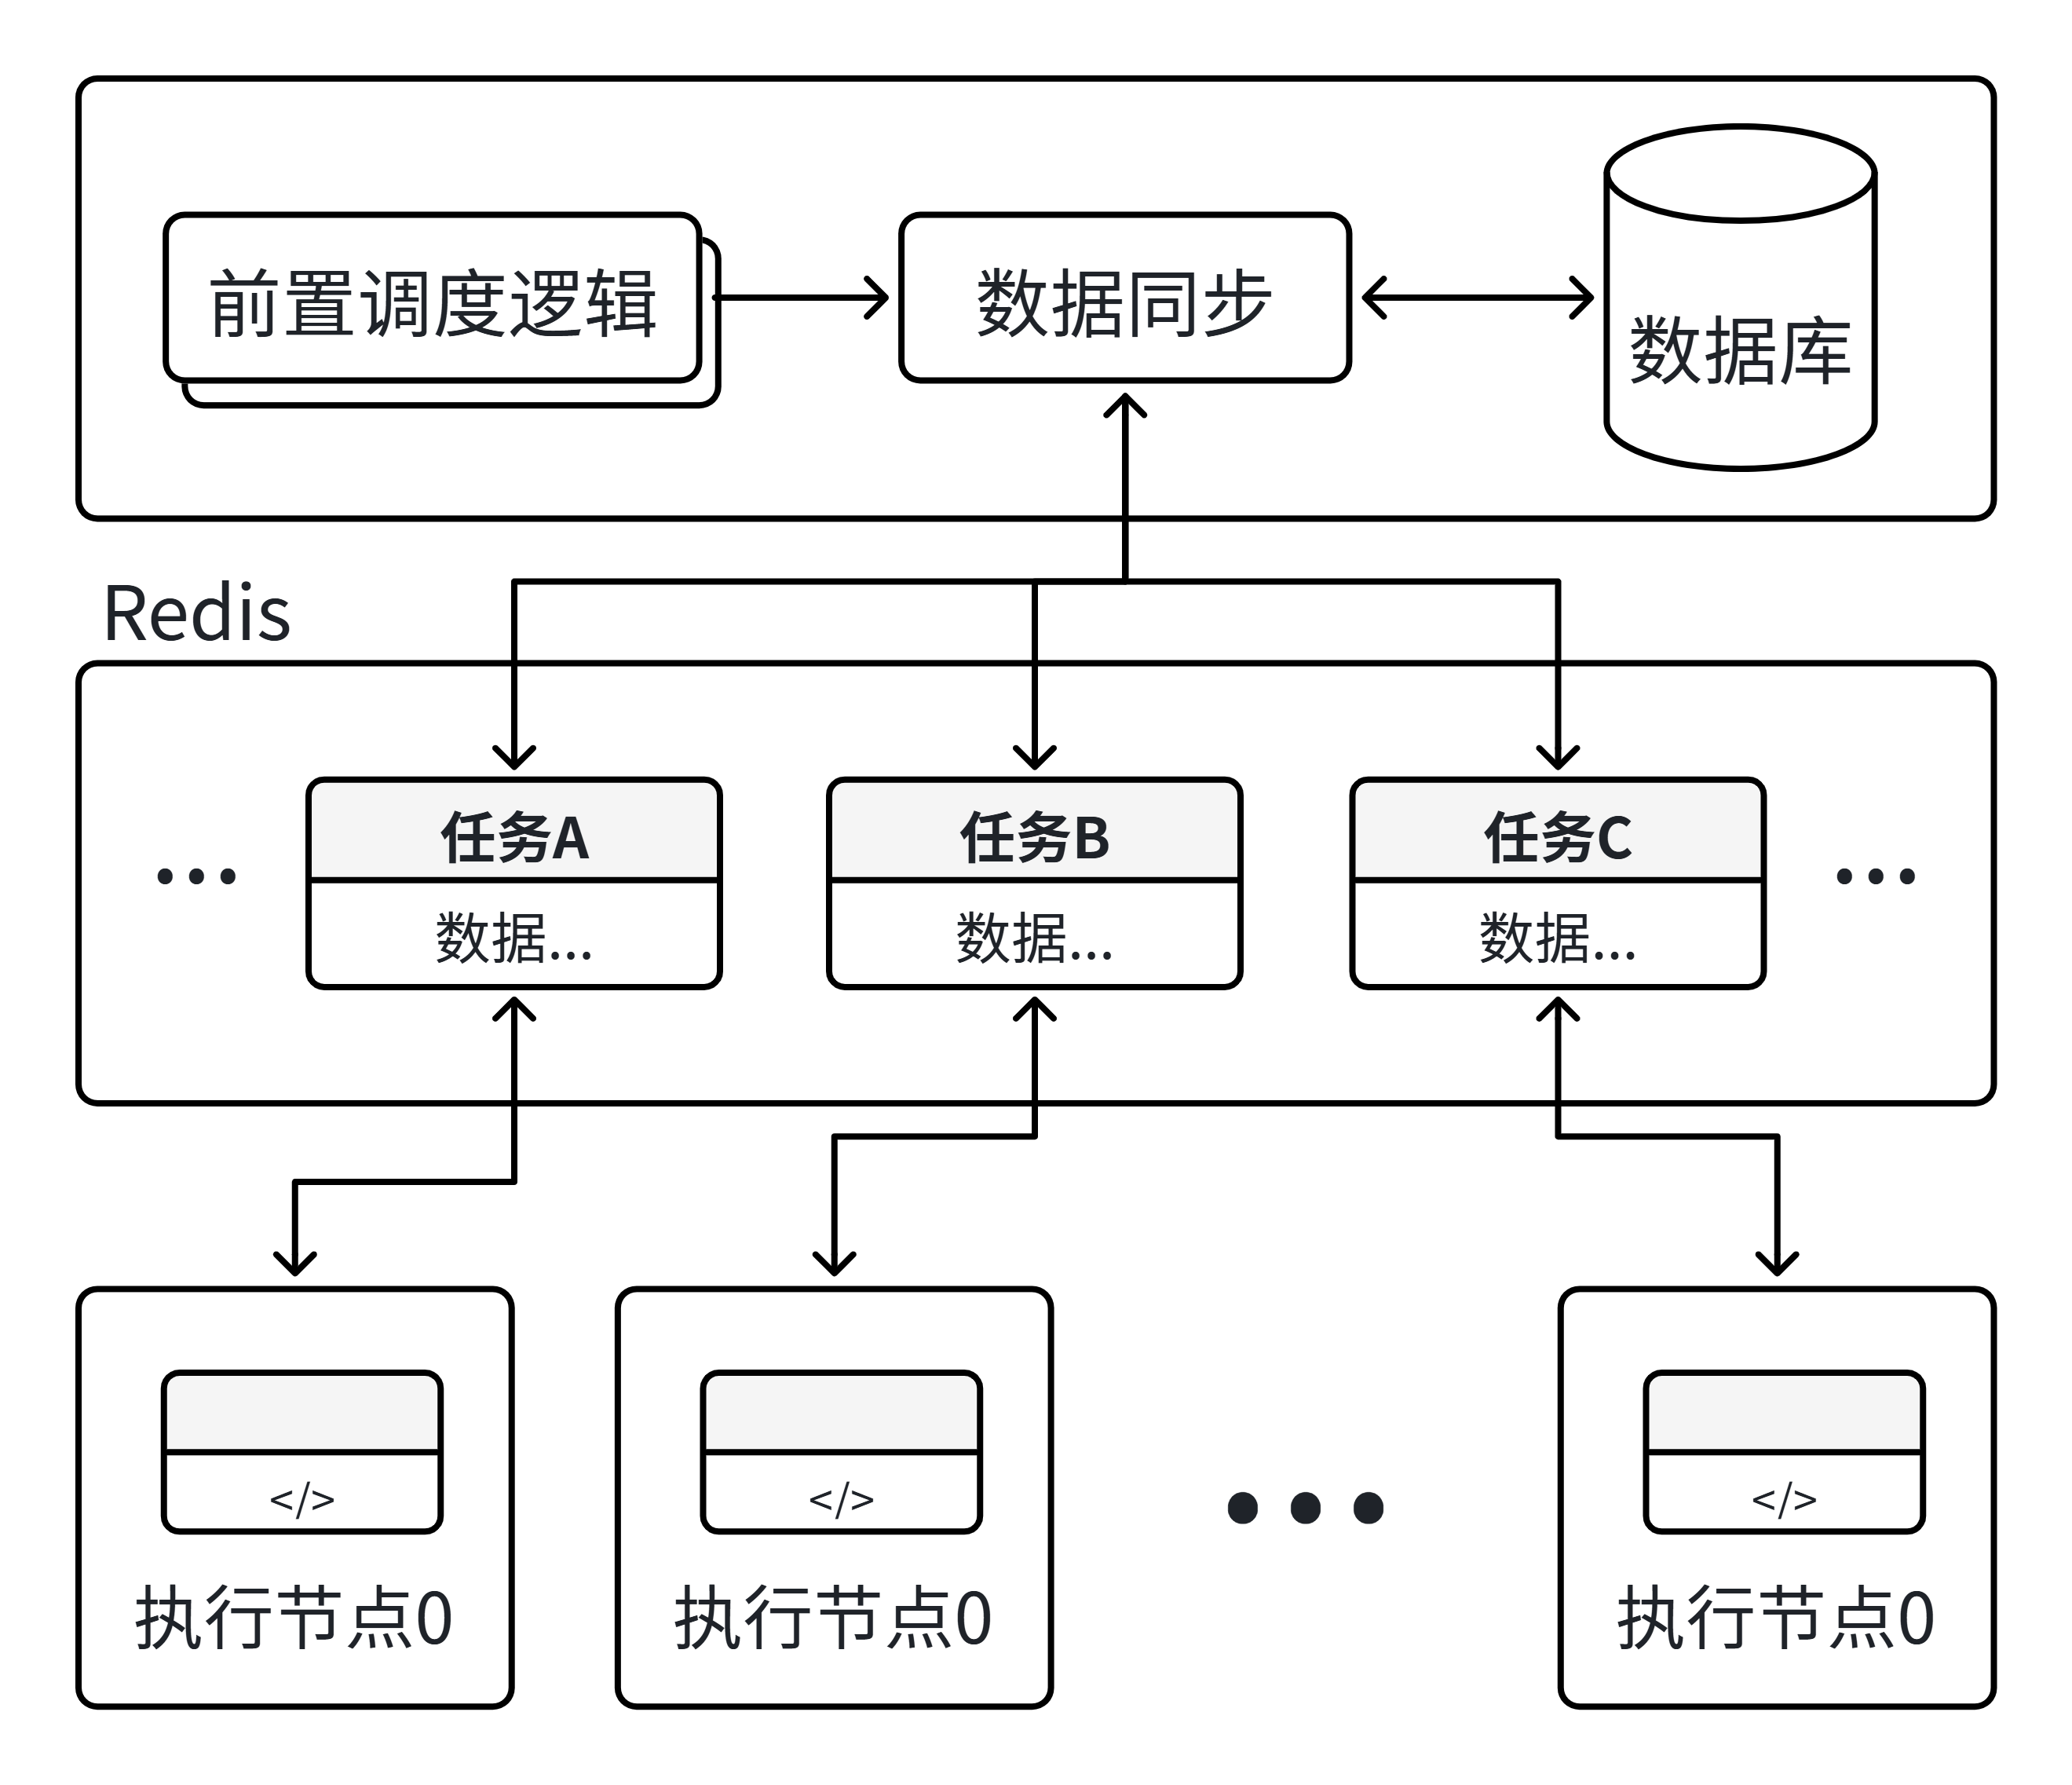
\includegraphics[width=\linewidth]{figures/5/数据同步模块原理图.png}
    \caption{数据同步模块原理图}
    \label{fig:enter-label}
\end{figure}

\subsection{容错与恢复机制}

本系统针对AI多任务场景下高算力消耗、执行周期长的特征，设计了一套具备环境感知能力的故障自愈机制。由于AI任务在执行过程中极易受到底层计算环境（如容器资源限制、网络波动等）的干扰导致异常中断，传统的调度模式往往需要操作员介入重提任务，造成了极高的人力和算力成本浪费。为此，系统通过构建全生命周期的指标监测体系，实现了对非致命性错误的自动化识别与闭环治理，旨在消除调度决策对人工干预的依赖，从底层保障算力资源的持续高效周转。

在技术落地层面，系统针对四类典型场景构建了精细化的自愈策略：首先，针对k8s环境下的CPU超限，系统在检测到限流抖动后会自动调低调度并发度，确保核心服务的可用性；其次，利用Python异常捕获机制识别内存不足（OOM）报错，系统会将受影响任务重置为等待状态并自动重回队列，待资源水位回落后执行异步调度，且支持最多三次的静默重试逻辑，重试间隔按照指数退避策略进行，三次重试均失败后，按照“执行失败”标记并推送面板，随即释放资源；再次，针对AI长周期任务中常见的文件描述符堆积，系统建立了实时监控与阈值预警机制，防止潜在的句柄泄露引发系统级崩溃；最后，面对网络抖动导致的API超时，系统内置了基于指数退避算法的重试策略，在保障任务执行韧性的同时有效规避了请求雪崩。通过这套多级容错体系，系统成功实现了从“人工排障”向“引擎自愈”的智能化转型。

\section{任务执行层详细设计}

作为系统算力落地的最终环节，任务执行层直接决定了AI多任务调度的响应质量与数据鲁棒性。针对现有系统在AI特性适配上的不足，本层通过构建标准化的路由分发机制与算子执行单元，确保调度中枢下发的智能化指令能精准转化为具体的算力输出。它不仅承担了繁重的异构数据处理工作，还与监控平台深度联动，通过对执行过程的实时感知，实现了从“参数流入”到“结果反馈”的全流程自动化管理，有效解决了因子模块环境差异导致的任务执行瓶颈。

路由模块在接收到调度平台下发的指令后，首先会启动关键的“环境初始化”程序。这一阶段不仅涵盖了针对大模型任务的异构数据映射，还深入涉及了模型参数的本地化预处理与张量对齐，旨在从执行端彻底化解子问题一中描述的多源异构适配难题。环境就绪后，路由模块将结合实时生成的任务画像（如算子偏好、显存预估等指标），动态挑选出最契合当前计算需求的执行算子，并正式驱动该算子开启高强度的AI计算任务。在任务运行的整个周期内，监控平台会建立高频采样通道，实时收集并统计算力节点的各项关键数据。系统能够精准捕获CPU利用率、显存带宽占用以及能耗分布等临界资源的动态变化，并将这些原始遥测数据转化为结构化的分析结果，实时反馈给路由模块以生成精炼的执行简报。最后，系统会将这份包含任务实时进度、性能水位线及异常拦截记录的简报同步至调度平台，从而在底层执行与上层调度之间形成了一个完整的状态反馈闭环。这种机制彻底告别了传统模式下依赖人工干预来监控任务状态的低效方式，使得大模型任务的整个执行过程在实现自动化流转的同时，变得既高效又透明。

具体的执行流程如图 5.10 所示。

\begin{figure}[htbp]
    \centering
    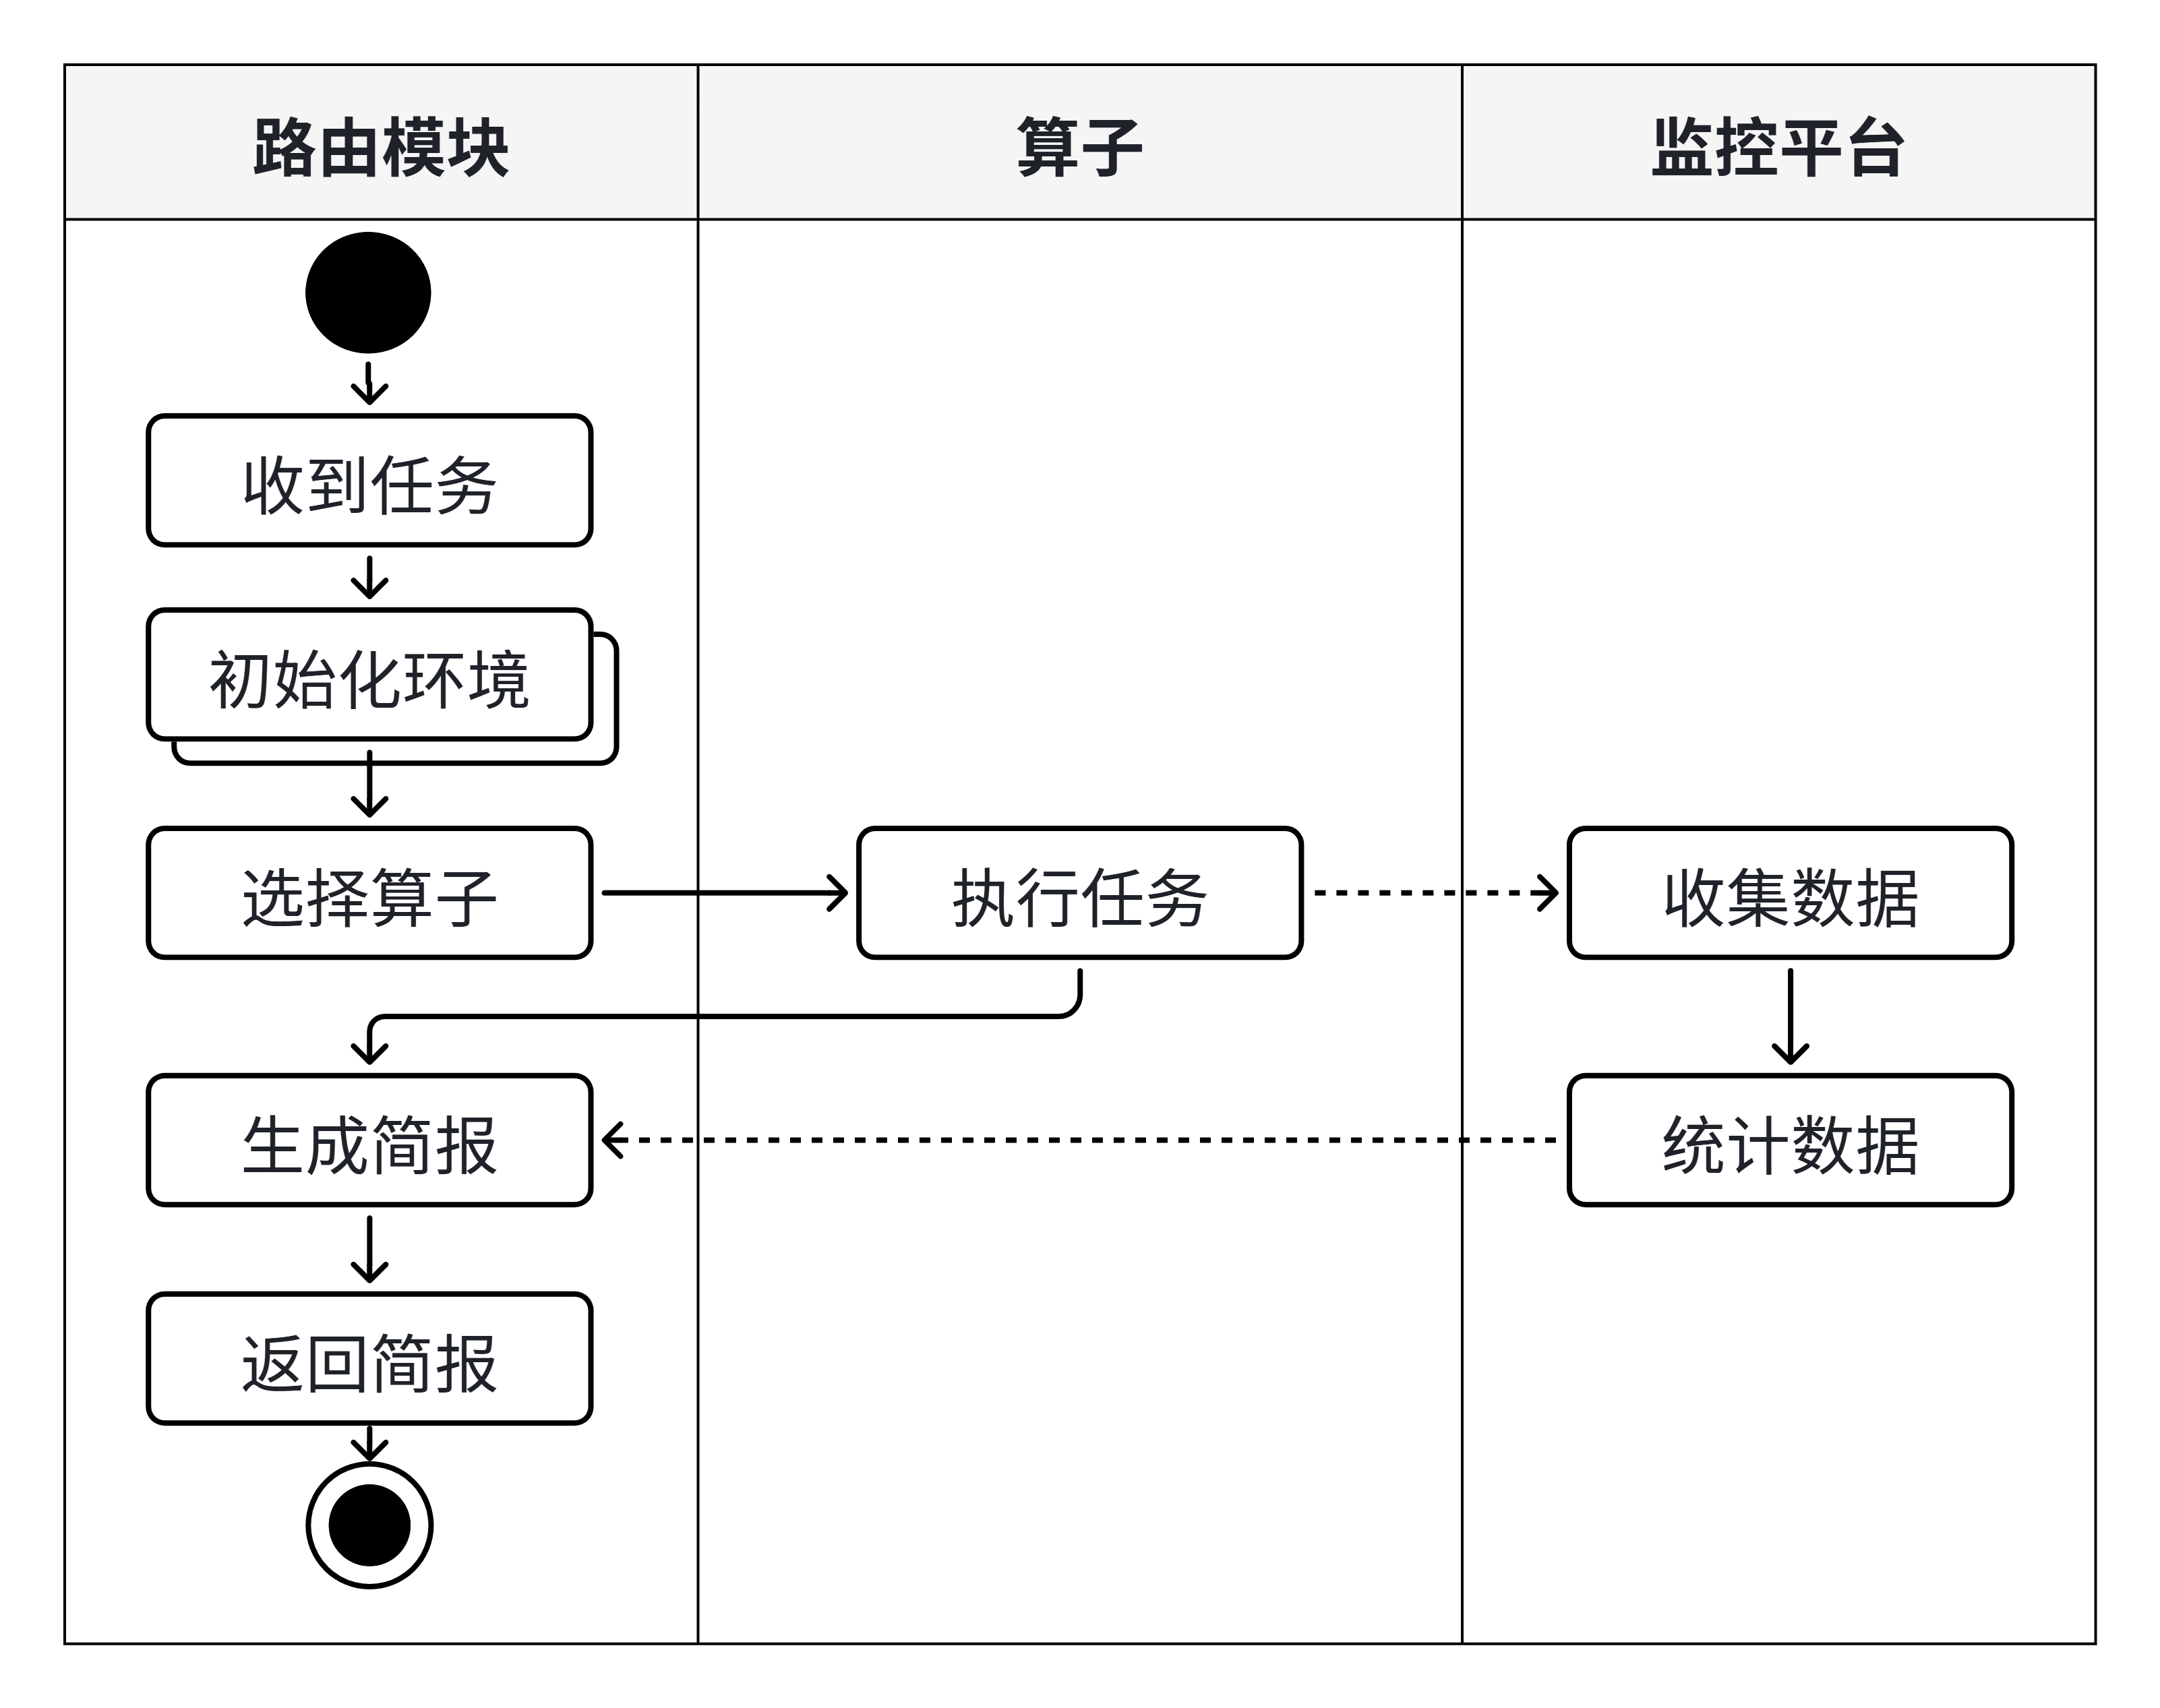
\includegraphics[width=\linewidth]{figures/5/任务执行流程.png}
    \caption{任务执行泳道图}
    \label{fig:enter-label}
\end{figure}

\subsection{参数传递约定}

本系统通过构建基于JSON与Python字典（dict）的深度映射机制，实现了AI异构参数在分布式环境下的透明流转。针对大模型任务参数多样、结构复杂的特性，这一设计充分发挥了Python生态与Celery框架在数据处理上的灵活性，从底层打通了前端面板、数据库与执行节点之间的信息链路。通过将非结构化的请求精准解析为逻辑层可识别的执行对象，系统不仅有效提升了对异构数据的处理兼容性，也为后续实现复杂的自动化调度决策奠定了统一的数据基准。

在具体实现细节上，系统规定了一套涵盖任务标识、资源链路及存储路径的基础参数协议。其中，resource\_url字段支持对AI依赖附件的自动化关联，而output\_dir与log\_dir则由系统根据任务画像自动生成并定向，彻底消除了过去需要程序员手动配置路径、预建目录的机械劳动，有效避免了因路径配置错误而导致的启动失败问题。此外，系统内置了参数合法性校验与运行环境自愈逻辑，在任务启动前会自动初始化物理目录，确保执行环境的一致性；在任务结束后，则会即时触发冗余数据清理机制，避免历史文件堆积对集群存储造成持续压力。这种从“自动创建”到“按需回收”的全流程管理模式，不仅显著降低了因子模块配置偏差导致的任务崩溃风险，也极大优化了算力集群的存储空间周转效率，为大规模任务的稳定调度奠定了可靠的基础设施支撑。参数传递约定如表5.3所示。

\begin{table}[htbp]
    \centering
    \caption{任务基本参数}
    \begin{tabular}{llllll}
        \toprule
        序号 & 字段名 & 字段说明 & 类型 & 是否可选 & 说明 \\
        \midrule
1 & task\_id & 任务ID & int & N &  \\
2 & celery\_id & Celery ID & int & N &  \\
3 & resource\_url & 所依赖资源链接 & string & Y & 任务可无附件 \\
4 & output\_dir & 任务输出文件路径 & string & N &  \\
5 & log\_dir & 任务日志路径 & string & N &  \\
        \bottomrule
    \end{tabular}
    \label{tab:my_label}
\end{table}

\subsection{任务编辑方式}

在AI大模型的研发迭代中，任务代码绝非一劳永逸，往往需要根据业务逻辑的演进或模型参数的调整进行动态修正。本系统针对传统模式下代码更新链路长、易出错的痛点，构建了一套涵盖“编辑、提交、审核、上线”四大环节的敏捷闭环机制。该机制旨在为操作员提供一条自动化的代码变更流水线，确保在保障系统运行环境一致性的前提下，能够快速、准确地修正业务逻辑。这不仅解决了手动更新带来的环境适配难题，也通过标准化的流程审计，进一步减少了由于代码误操作导致的算力资源空耗，为实现调度决策的自动化提供了可靠的逻辑底座。

在具体工程实现上，代码变更流程被赋予了极强的容错与安全属性。操作员在完成代码针对性修订的同时，系统会同步采集配套的依赖库信息，通过自动化构建保障执行端环境的无偏差映射，确保开发环境与生产环境在依赖层面保持严格一致，从根本上杜绝了因“本地跑得通、线上崩了”引发的执行异常。为了筑牢安全防线，系统引入了管理员审计机制，所有待发布的代码变更与依赖更新均需经过管理员的严格审查与确认，通过对逻辑变更与依赖更新的双重审核，有效拦截潜在的运行风险。一旦审核通过，全自动分发引擎会即时将新代码推送到分布式执行节点，实现业务逻辑的无感升级，整个过程对正在运行的任务无任何干扰。更为关键的是，系统依托Git技术设计了线性版本管理策略，为每一次代码更替配置了“一键回滚”的兜底手段。当新代码出现非预期行为时，操作人员可迅速撤回至历史稳定版本，将故障影响控制在最小范围内。这种“自动化部署+版本化隔离”的设计，不仅解决了AI多任务场景下的频繁迭代难题，也极大提升了系统的整体韧性与运维效率，为持续交付提供了可靠的技术保障。任务编辑的垂直泳道图如图5.11所示。

\begin{figure}[htbp]
    \centering
    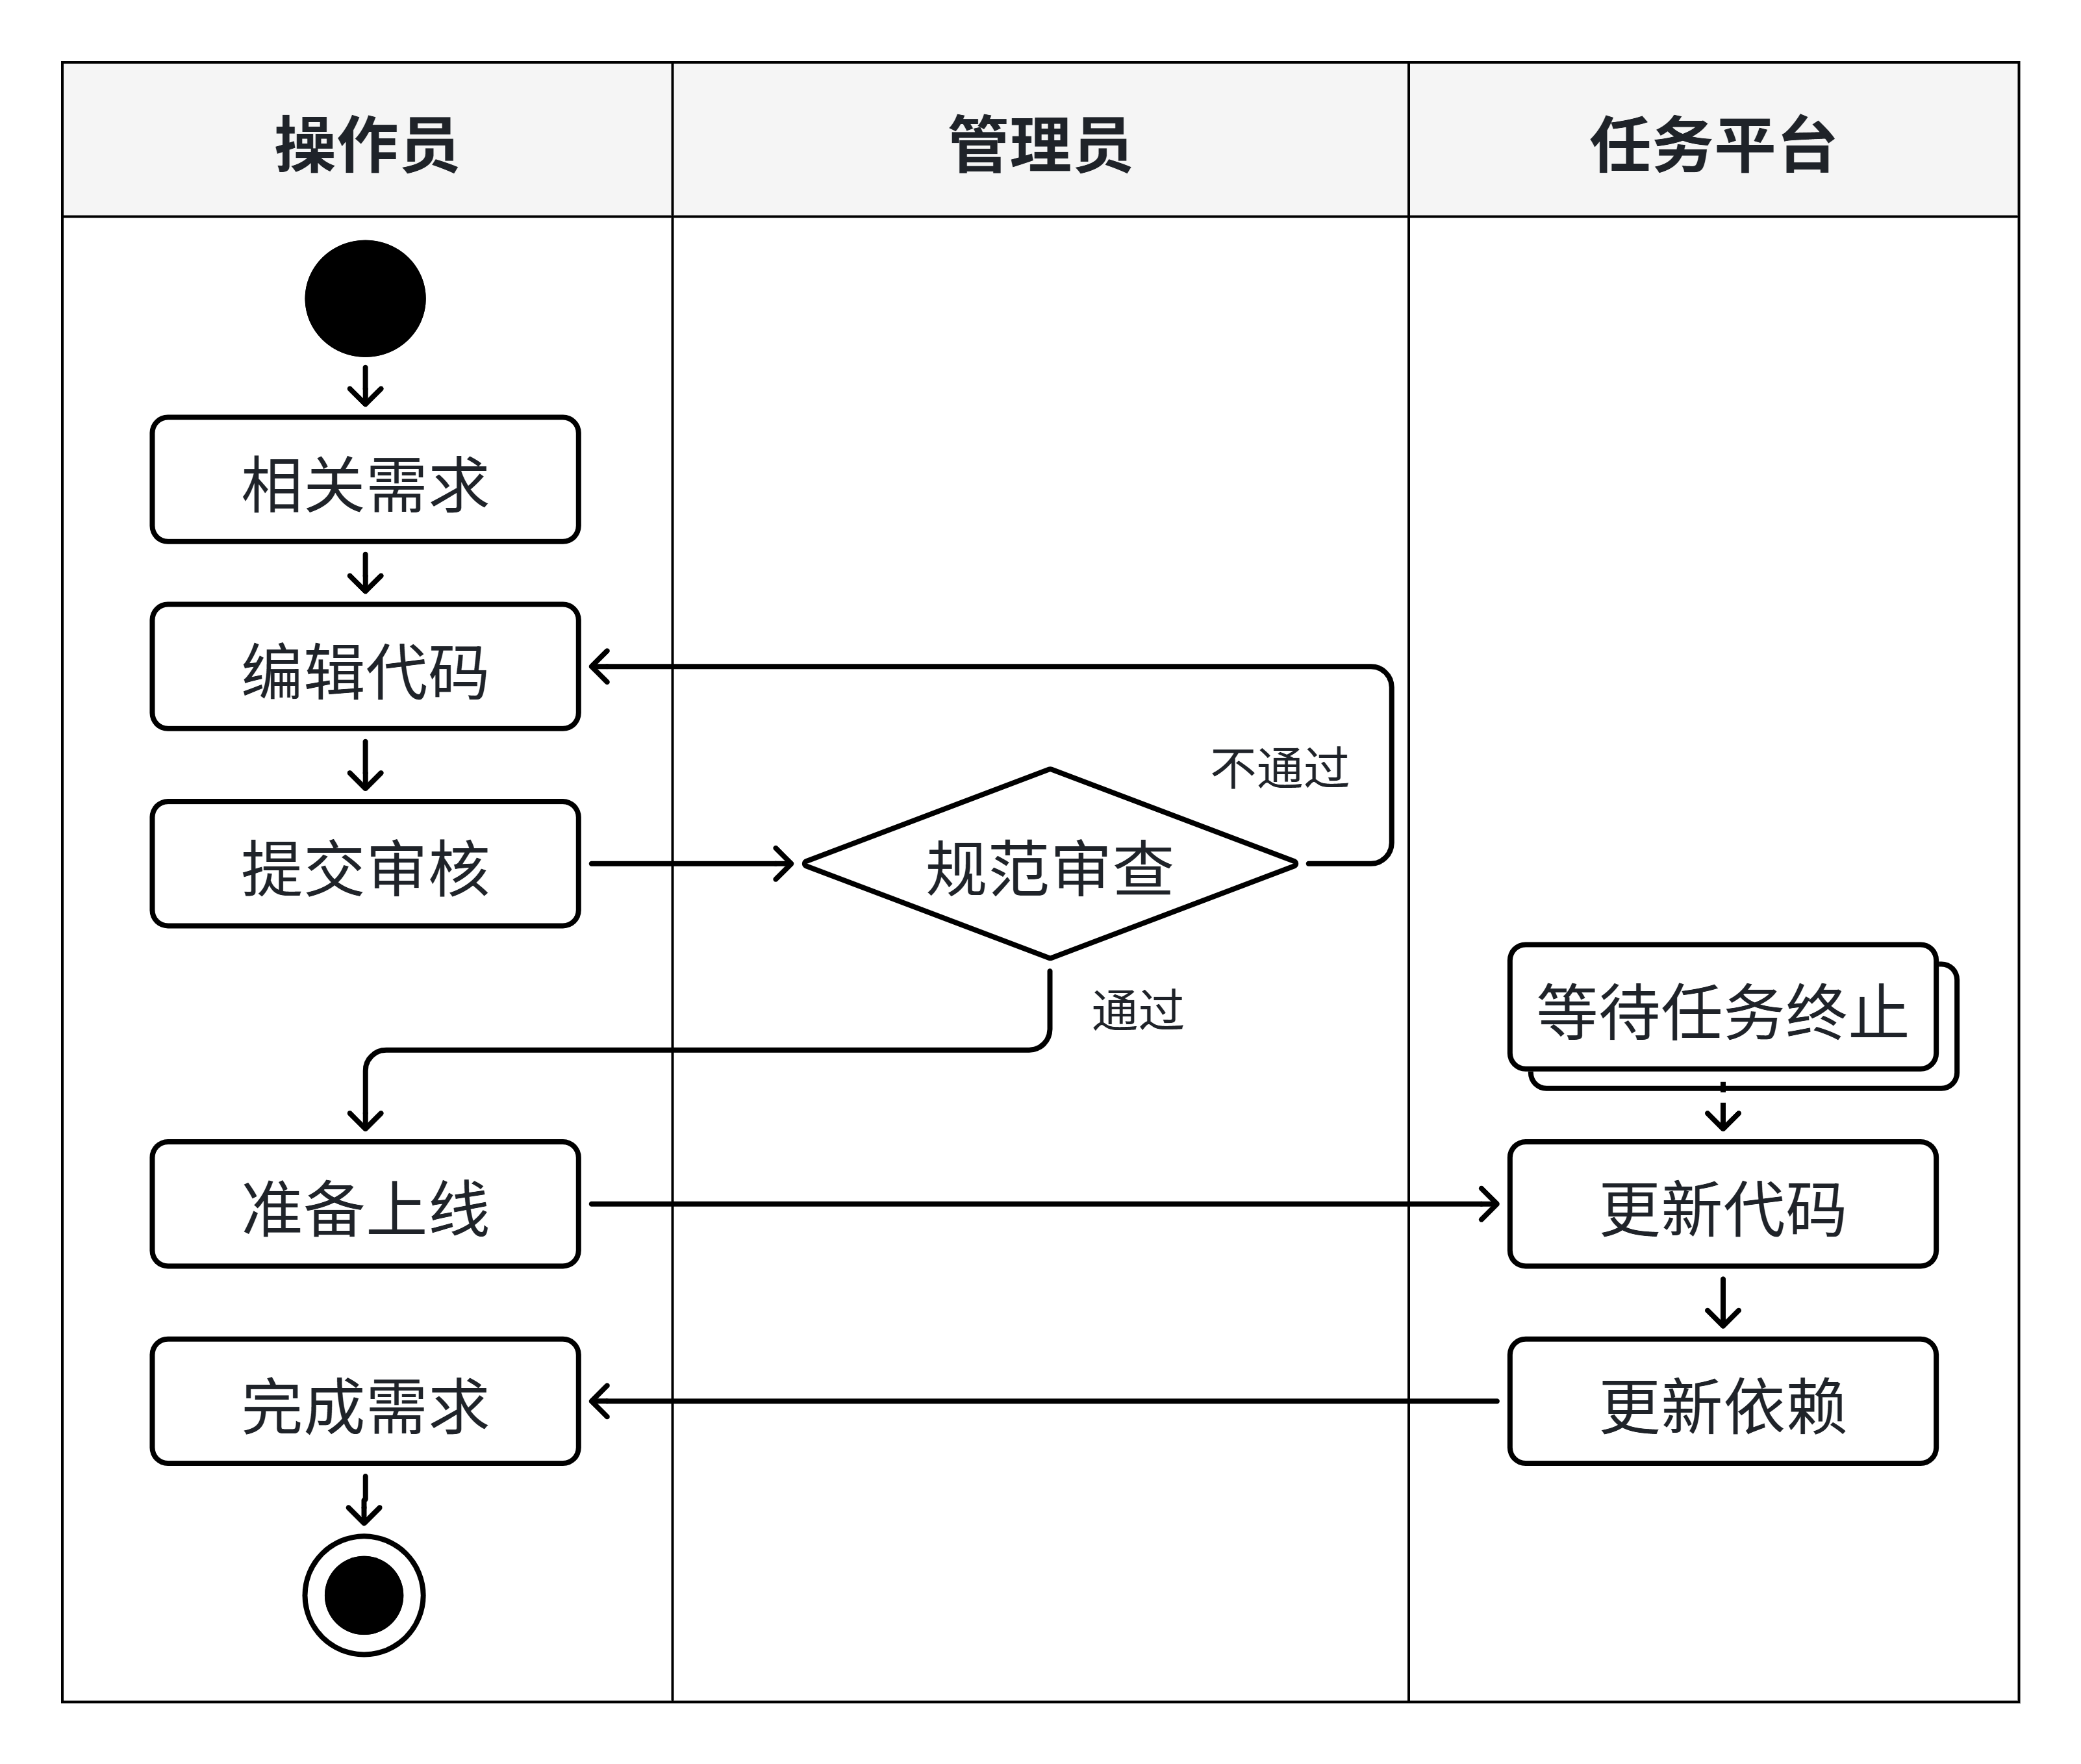
\includegraphics[width=\linewidth]{figures/5/任务编辑垂直泳道图.png}
    \caption{任务编辑泳道图}
    \label{fig:enter-label}
\end{figure}

\subsection{异常捕获机制}

本层异常捕获机制的设计，主要是为配合上文任务调度层中的容错与恢复机制而使用，旨在通过及时捕获并处理异常，为调度层的容错策略提供支持，确保系统在出现问题时能够高效执行恢复操作，提升整体运行的稳定性。任务调度层“容错与恢复机制”的核心功能是对本层抛出的异常进行判断、分析与恢复，故本层的主要职责则是精准抛出异常，并附带完整的调试与纠错信息，为上层的准确判断提供依据。这种分层协作机制，通过明确的功能划分，确保异常从捕获到处理的全流程高效衔接 —— 本层负责 “精准输出问题”，上层专注 “高效解决问题”，二者形成闭环，有效提升了系统应对故障的响应速度与处理精度。

从实际运行来看，本层抛出的异常信息越详尽，任务调度层的恢复策略就越具针对性。例如，当检测到资源占用超限的异常时，本层会同步上传资源使用曲线、进程 ID 等关键数据，调度层便能据此快速定位冲突进程，而非盲目重启系统，这也体现了分层设计在系统稳定性保障中的关键价值。由于不同任务需要向系统提交的异常信息存在差异，因此本机制处于持续开发迭代的状态。操作员在部署新的任务代码前，可向系统开发者提出需求，要求监测额外信息；开发者接到需求后，会对系统进行改进，以满足操作员对任务监控信息的需求。一般而言，新增一个监控指标的工作量相对有限，相应的迭代开发周期约为半天，因此不会对任务交付进度造成显著影响。本系统任务执行模块异常处理流转状态机如图5.12所示。

\begin{figure}[htbp]
    \centering
    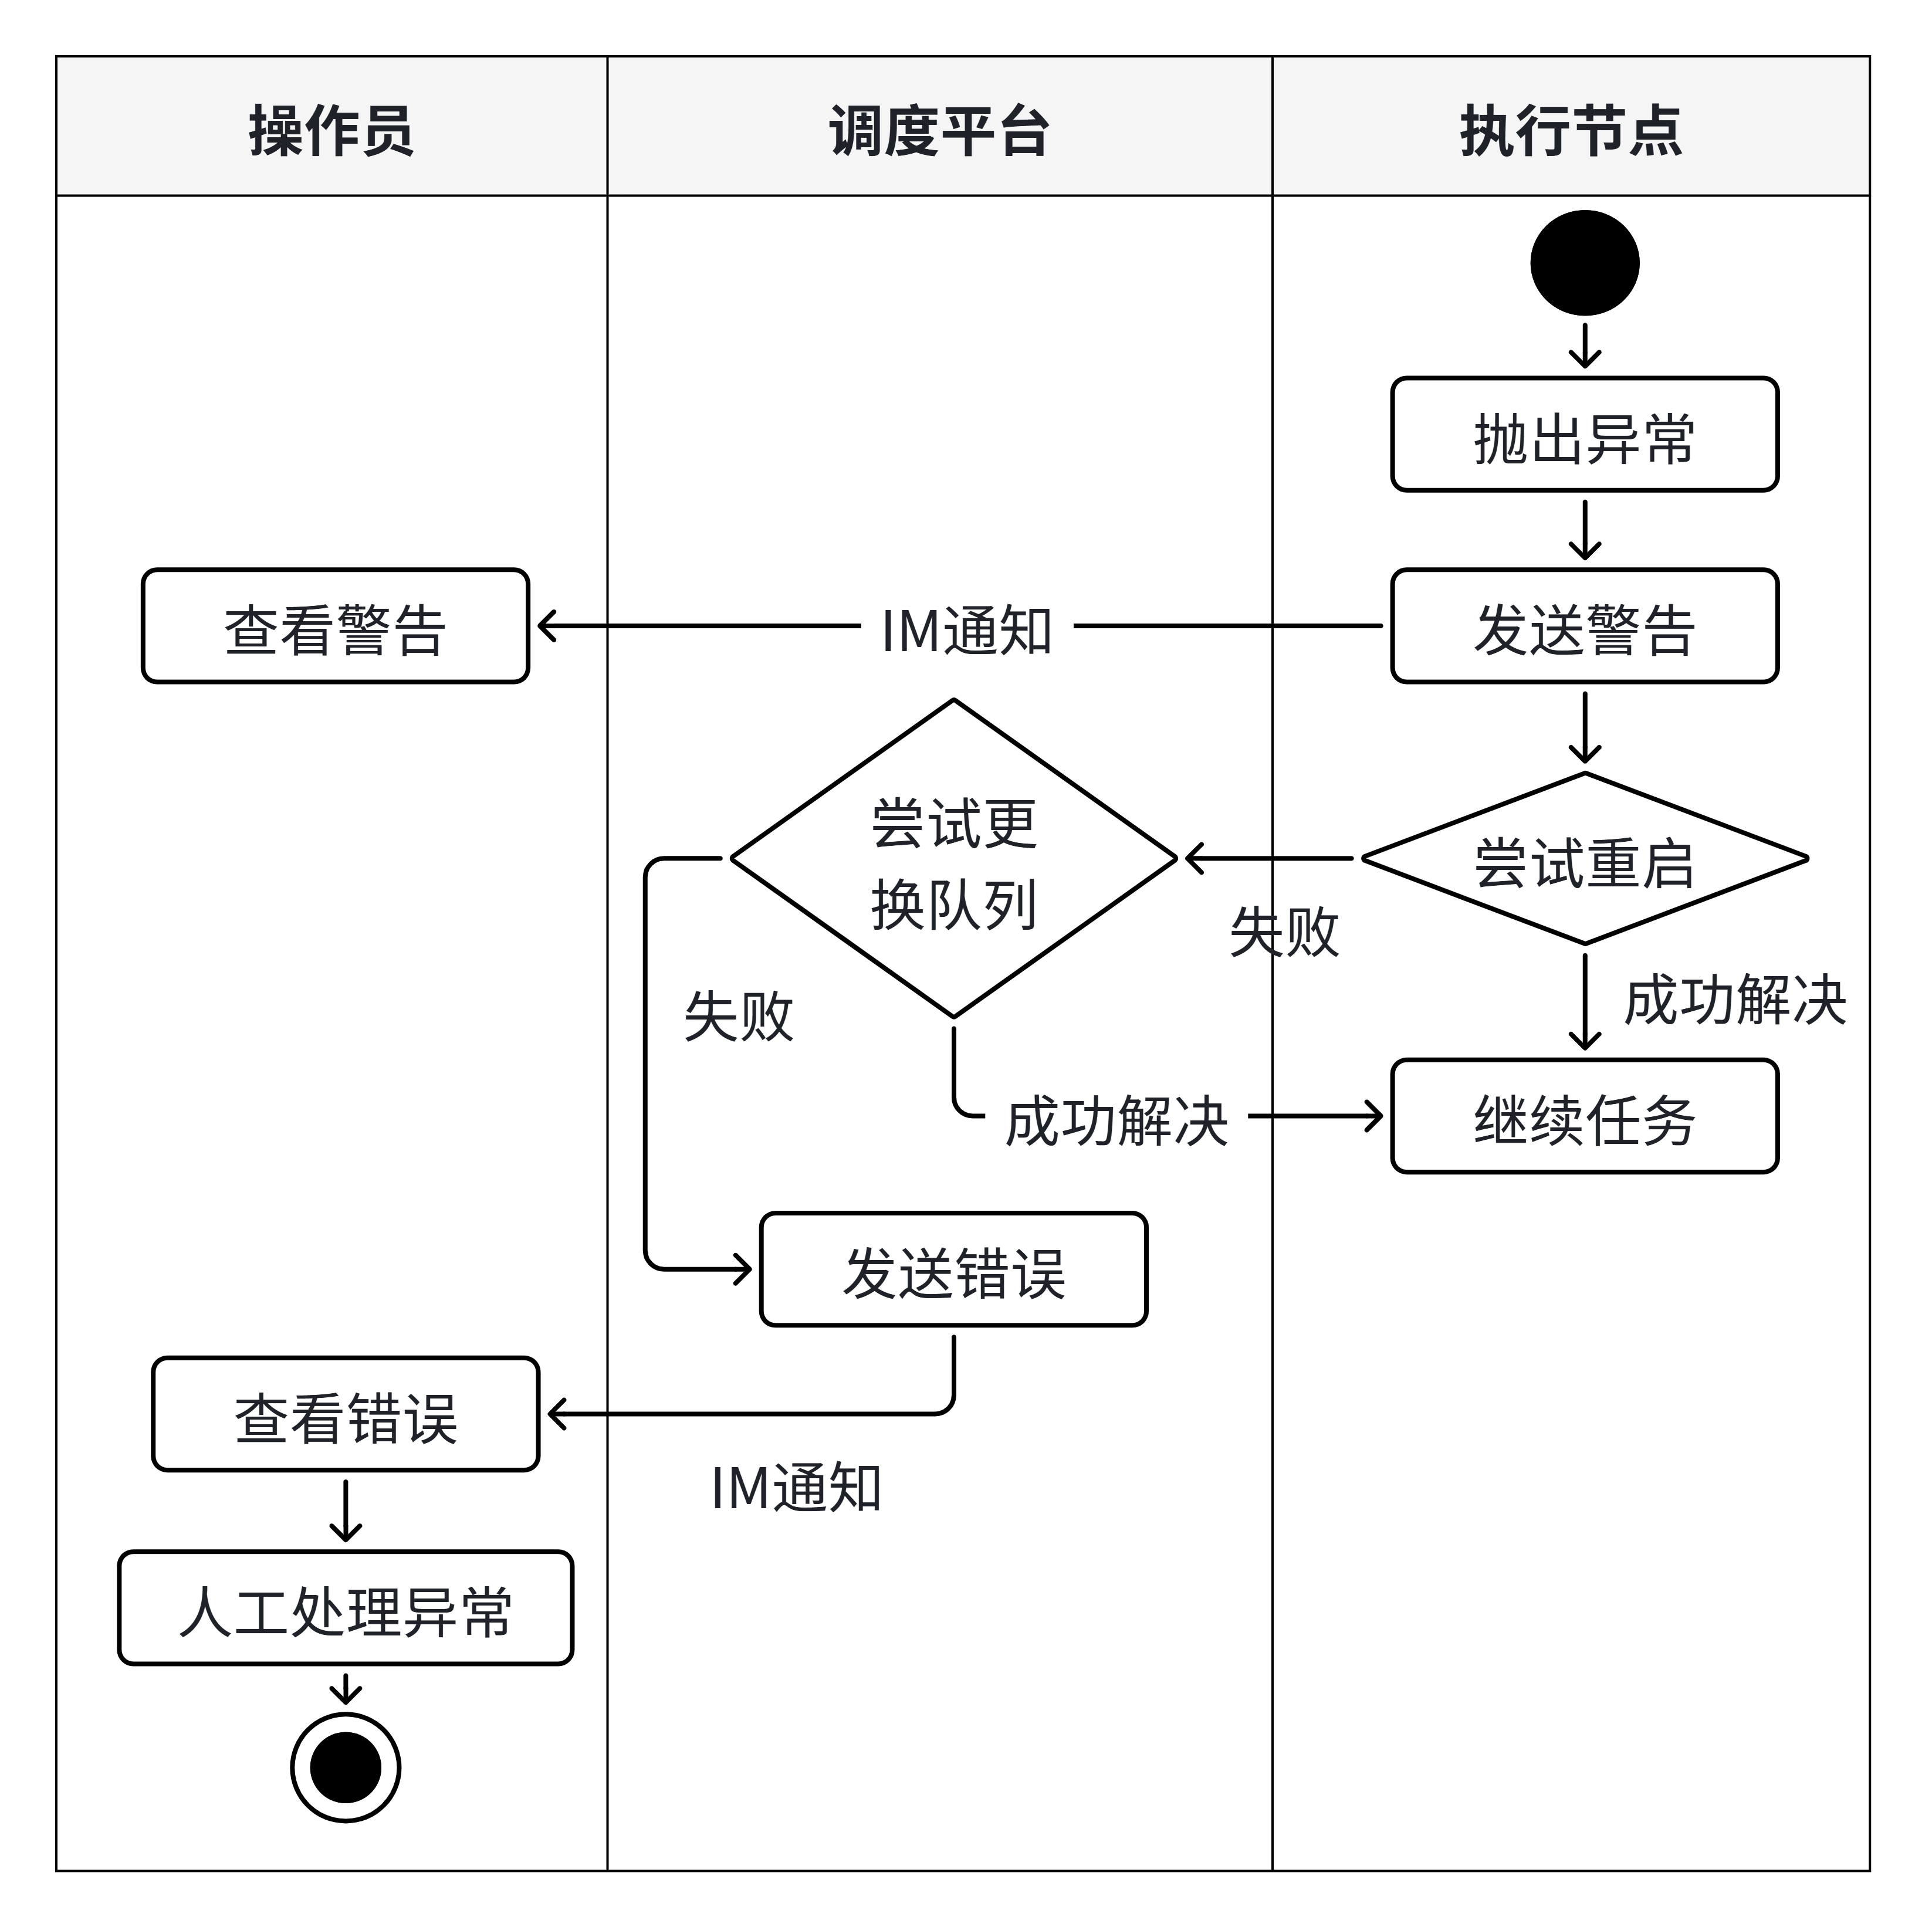
\includegraphics[width=\linewidth]{figures/5/异常处理状态流转.png}
    \caption{异常处理状态流转泳道图}
    \label{fig:enter-label}
\end{figure}

\section{系统总体工作流程}

流程从操作员开始。操作员通过网页操作并填入参数，向调度平台Web端发送请求。调度平台Web端接收到请求后，进行HTTP 请求处理。随后，请求进入调度平台服务器。在调度平台服务器内，请求处理过程分为多个步骤。首先是鉴权请求，确保请求来源的合法性和安全性。接着进行初步处理，对请求进行初步分析和准备。然后是调度算法，通过预设的算法逻辑，确定任务的优先级、资源分配和执行顺序等关键因素。调度算法完成后，进行任务路由，即将任务分配到合适的执行队列中。最后，任务执行队列负责执行任务，确保任务按照预定的计划和要求顺利完成。

\section{本章小结}

本章围绕AI调度三大问题展开详细设计与实现。针对AI特性适配不佳、操作复杂的问题，API接入层通过权限鉴定模块和数据校验模块简化操作、提升适配性；针对无法判断任务执行条件、依赖人工的问题，任务调度层设计任务可用性检测机制与状态机，结合数据同步模块实现任务自动调度；针对无法识别资源互斥的问题，通过资源可用性检测与负载均衡算法优化资源分配，搭配容错恢复与异常捕获机制保障稳定。同时任务执行层明确参数传递与代码管理流程，整体构建起覆盖API、调度、执行的系统架构。

\makeatletter
\@openrightfalse
\makeatother